%%%%%%%%%%%%%%%%%%%%%%%%%%%%%%%%%%%%%%%%%
% Masters/Doctoral Thesis 
% LaTeX Template
% Version 2.4 (22/11/16)
%
% This template has been downloaded from:
% http://www.LaTeXTemplates.com
%
% Version 2.x major modifications by:
% Vel (vel@latextemplates.com)
%
% This template is based on a template by:
% Steve Gunn (http://users.ecs.soton.ac.uk/srg/softwaretools/document/templates/)
% Sunil Patel (http://www.sunilpatel.co.uk/thesis-template/)
%
% Template license:
% CC BY-NC-SA 3.0 (http://creativecommons.org/licenses/by-nc-sa/3.0/)
%
%%%%%%%%%%%%%%%%%%%%%%%%%%%%%%%%%%%%%%%%%

%----------------------------------------------------------------------------------------
%	PACKAGES AND OTHER DOCUMENT CONFIGURATIONS
%----------------------------------------------------------------------------------------

\documentclass[
11pt, % The default document font size, options: 10pt, 11pt, 12pt
oneside, % Two side (alternating margins) for binding by default, uncomment to switch to one side
english, % ngerman for German
doublespacing, % Single line spacing, alternatives: onehalfspacing or doublespacing
%draft, % Uncomment to enable draft mode (no pictures, no links, overfull hboxes indicated)
%nolistspacing, % If the document is onehalfspacing or doublespacing, uncomment this to set spacing in lists to single
%liststotoc, % Uncomment to add the list of figures/tables/etc to the table of contents
%toctotoc, % Uncomment to add the main table of contents to the table of contents
%parskip, % Uncomment to add space between paragraphs
%nohyperref, % Uncomment to not load the hyperref package
headsepline, % Uncomment to get a line under the header
%chapterinoneline, % Uncomment to place the chapter title next to the number on one line
%consistentlayout, % Uncomment to change the layout of the declaration, abstract and acknowledgements pages to match the default layout
]{MastersDoctoralThesis} % The class file specifying the document structure

\usepackage[utf8]{inputenc} % Required for inputting international characters
\usepackage[T1]{fontenc} % Output font encoding for international characters
\usepackage{amssymb,amsmath}
\usepackage{physics}
\usepackage{titlesec}
\usepackage{caption}
\usepackage{subcaption}
\newcommand{\sectionbreak}{\clearpage}
\usepackage{nameref}
\usepackage{palatino} % Use the Palatino font by default

\usepackage[backend=biber,style=numeric,natbib=true]{biblatex} % Use the bibtex backend with the authoryear citation style (which resembles APA)

\addbibresource{example.bib} % The filename of the bibliography

\usepackage[autostyle=true]{csquotes} % Required to generate language-dependent quotes in the bibliography

%----------------------------------------------------------------------------------------
%	MARGIN SETTINGS
%----------------------------------------------------------------------------------------
\geometry{
	paper=a4paper, % Change to letterpaper for US letter
	inner=2.5cm, % Inner margin
	outer=3.8cm, % Outer margin
	bindingoffset=.5cm, % Binding offset
	top=1.5cm, % Top margin
	bottom=1.5cm, % Bottom margin
	%showframe, % Uncomment to show how the type block is set on the page
}

%----------------------------------------------------------------------------------------
%	THESIS INFORMATION
%----------------------------------------------------------------------------------------

\thesistitle{3D Superconducting Transmon Qubit} % Your thesis title, this is used in the title and abstract, print it elsewhere with \ttitle
\supervisor{\href{http://www.physics.iisc.ernet.in/~v.singh/}{\color{black}{Dr. Vibhor Singh\\ Assistant Professor, IISc Bangalore}}} % Your supervisor's name, this is used in the title page, print it elsewhere with \supname
\examiner{} % Your examiner's name, this is not currently used anywhere in the template, print it elsewhere with \examname
\degree{M.Sc. (Hons.) Physics} % Your degree name, this is used in the title page and abstract, print it elsewhere with \degreename
\author{Rohit H Navarathna} % Your name, this is used in the title page and abstract, print it elsewhere with \authorname
\addresses{} % Your address, this is not currently used anywhere in the template, print it elsewhere with \addressname

\subject{Physicsl Sciences} % Your subject area, this is not currently used anywhere in the template, print it elsewhere with \subjectname
\keywords{} % Keywords for your thesis, this is not currently used anywhere in the template, print it elsewhere with \keywordnames
\university{\href{http://www.bits-pilani.ac.in/Goa/}{\color{black}{BITS, PILANI –K K BIRLA GOA CAMPUS}}} % Your university's name and URL, this is used in the title page and abstract, print it elsewhere with \univname
\department{} % Your department's name and URL, this is used in the title page and abstract, print it elsewhere with \deptname
\group{} % Your research group's name and URL, this is used in the title page, print it elsewhere with \groupname
\faculty{} % Your faculty's name and URL, this is used in the title page and abstract, print it elsewhere with \facname

\AtBeginDocument{
\hypersetup{pdftitle=\ttitle} % Set the PDF's title to your title
\hypersetup{pdfauthor=\authorname} % Set the PDF's author to your name
\hypersetup{pdfkeywords=\keywordnames} % Set the PDF's keywords to your keywords
}

\begin{document}

\frontmatter % Use roman page numbering style (i, ii, iii, iv...) for the pre-content pages

\pagestyle{plain} % Default to the plain heading style until the thesis style is called for the body content

\newcommand{\JJ}{Josephson Junction }
\newcommand{\CPB}{Cooper Pair Box }

%----------------------------------------------------------------------------------------
%	TITLE PAGE
%----------------------------------------------------------------------------------------

\begin{titlepage}
\begin{center}
\HRule \\[0.4cm] % Horizontal line
{\huge \bfseries \ttitle\par}\vspace{0.4cm} % Thesis title
\HRule \\[1.5cm] % Horizontal line

\textsc{\Large THESIS}\\[0.5cm] % Thesis type
\large \textit{Submitted in partial fulfillment of the requirements of\\\textbf{BITS F421T, Thesis}}\\[0.3cm] % University requirement text
%\vspace*{.06\textheight}
by\vspace{0.5cm}


\Large{\authorname}\\% Author name - remove the \href bracket to remove the link
ID No - 2013B5TS364G\\\vspace{1.5cm}
\large Under the supervision of\\\vspace{0.5cm}
\Large{\supname} % Supervisor name - remove the \href bracket to remove the link
 
\vfill

\includegraphics[width=6cm]{Figures/Logo.png}\\ % University/department logo - uncomment to place it
{\scshape\LARGE \textbf{\univname}\par}\vspace{1.5cm} % University name
\vfill
\end{center}
\end{titlepage}
%----------------------------------------------------------------------------------------
%	ABSTRACT PAGE
%----------------------------------------------------------------------------------------

\begin{abstract}
\addchaptertocentry{\abstractname} % Add the abstract to the table of contents
Superconducting Qubits are a promising candidate for quantum computing. The use of a high quality 3D superconducting cavity to interact with a \JJ qubit greatly increases it's coherence time. Shunting the \JJ with a large capacitance decreases charge noise exponentially while maintaining the necessary anharmonicity to access only 2 levels of the system. Microwave signals of appropriate frequency can be used to cause Rabi oscillations in the qubit and control it's quantum state. The $S_{11}$ response of the cavity reveals the state of the qubit when they are dispersively coupled. The coherence time and time scales that manipulate the qubit can be estimated using this response.
\end{abstract}

%----------------------------------------------------------------------------------------
%	ACKNOWLEDGEMENTS
%----------------------------------------------------------------------------------------

\begin{acknowledgements}
\addchaptertocentry{\acknowledgementname} % Add the acknowledgements to the table of contents
I would like to thank the Academic Research Division in Birla Institute of Technology and Science, KK Birla Goa Campus for giving me this great opportunity.
 
I would also like to thank my thesis advisor Dr. Vibhor Singh at the Indian Institute of Science, Bangalore. His guidance always helped me in writing this thesis. He consistently allowed this thesis to be my own work, but steered me in the right the direction whenever he thought I needed it.

I thank my fellow labmates in the Quantum-NEMS Group: Sudhir Kumar Sahu, Sourav Majumder, Soumya Ranjan Das, Dr.Bindumalini Gunupudi and Soma Mishra for the stimulating discussions and the knowledge they shared with me.

Last but not the least, I would like to thank my family, especially my parents for supporting me throughout this thesis and my life.
\end{acknowledgements}

%----------------------------------------------------------------------------------------
%	LIST OF CONTENTS/FIGURES/TABLES PAGES
%----------------------------------------------------------------------------------------

\tableofcontents % Prints the main table of contents

\listoffigures % Prints the list of figures

\listoftables % Prints the list of tables

%----------------------------------------------------------------------------------------
%	ABBREVIATIONS
%----------------------------------------------------------------------------------------

\begin{abbreviations}{ll} % Include a list of abbreviations (a table of two columns)

\textbf{AC} & \textbf{A}lternating \textbf{C}urrent\\
\textbf{BCS} & \textbf{B}ardeen \textbf{C}ooper and \textbf{S}chrieffer \\
\textbf{FWHM} & \textbf{F}ull \textbf{W}idth at \textbf{H}alf \textbf{M}aximum\\
\textbf{HEMT} & \textbf{H}igh \textbf{E}lectron \textbf{M}obility \textbf{T}ransistor\\
\textbf{QED} & \textbf{Q}uantum \textbf{E}lectro-\textbf{D}ynamics\\
\textbf{QND} & \textbf{Q}uantum \textbf{N}on \textbf{D}emolition\\
\textbf{SHO} & \textbf{S}imple \textbf{H}armonic \textbf{O}scillator\\
\textbf{SIS} & \textbf{S}uperconductor-\textbf{I}nsulator-\textbf{S}uperconductor\\\textbf{TE} & \textbf{T}ransverse \textbf{E}lectric\\
\textbf{TEM} & \textbf{T}ransverse \textbf{E}lectric and \textbf{M}agnetic\\
\textbf{TM} & \textbf{T}ransverse \textbf{M}agnetic\\
\textbf{VNA} & \textbf{V}ector \textbf{N}etwork \textbf{A}nalyser\\

\end{abbreviations}

%----------------------------------------------------------------------------------------
%	PHYSICAL CONSTANTS/OTHER DEFINITIONS
%----------------------------------------------------------------------------------------

\begin{constants}{lr@{${}={}$}l} % The list of physical constants is a three column table

% The \SI{}{} command is provided by the siunitx package, see its documentation for instructions on how to use it

Speed of Light & $c_{0}$ & \SI{2.99792458e8}{\meter\per\second} (exact)\\
Reduced Planks Constant & $\hbar$ & \SI{1.054571800e-34}{\joule\second} \\
Planks Constant & $h$ & \SI{6.62607004e-34}{\joule\second} \\
Elementary Charge & $e$ & \SI{1.60217662e-19}{\coulomb}\\
Magnetic Flux Quantum & $\Phi_0$ & \SI{2.067833831e-15}{\weber} \\
Boltzmann Constant & $k_B$ & \SI{1.38064852e-23}{\joule\per\kelvin} \\
Pi & $\pi$ & \SI{3.14159265359}{} \\
%Constant Name & $Symbol$ & $Constant Value$ with units\\

\end{constants}

%----------------------------------------------------------------------------------------
%	SYMBOLS
%----------------------------------------------------------------------------------------

\begin{symbols}{lll} % Include a list of Symbols (a three column table)
&\Large{\textbf{\nameref{Chapter2}}}\\
 \\
$C$ & Capacitance & \si{\farad}\\
$\bar{E}$ & Electric Field & \si{\volt\per\meter} \\
$\bar{H}$ & Magnetic Field & \si{\tesla} \\
$k$ & Wave Number & \si{\per\meter}\\
$L$ & Inductance & \si{\henry}\\
$Q$ & Quality Factor & \si{}\\
$Q_c$ & Coupling Quality Factor & \si{}\\
$Q_i$ & Internal Quality Factor & \si{}\\
$Q_t$ & Total (Loaded) Quality Factor & \si{}\\
$R$ & Resistance & \si{\ohm}\\
$S_{ij}$ & Scattering Parameter & \si{}\\
$v_p$ & Phase Velocity & \si{\meter\per\second}\\
$Z$ & Impedance & \si{\ohm}\\
 \\
$\alpha$ & Attenuation & \si{} \\
$\beta$ & Propogation Constant & \si{} \\
$\gamma$ & $\alpha+j\beta$ & \si{} \\
$\epsilon$ & Electric Permittivity & \si{\farad\per\meter}\\
$\epsilon_r$ & Relative Electric Permittivity & \si{}\\
$\eta$ & Intrinsic Impedance & \si{\ohm}\\
$\kappa$ & Cavity Decay Rate & \si{\hertz}\\
$\kappa_e$ & External Cavity Coupling Rate & \si{\hertz}\\
$\kappa_i$ & Internal Cavity Coupling Rate & \si{\hertz}\\
$\mu$ & Magnetic Permeability & \si{\henry\per\meter}\\
$\mu_r$ & Relative Magnetic Permeability & \si{}\\
$\sigma$ & Electric Conductivity & \si{\siemens\per\ohm}\\
$\omega$ & Angular Frequency & \si{\radian\per\second} \\
$\omega_0$ & Resonance Frequency & \si{\radian\per\second} \\
 \\
&\Large{\textbf{\nameref{Chapter3}}}\\
 \\
$a$ & Annihilation,Amplitude Operator & \si{}\\
$a^\dag$ & Creation Operator & \si{}\\
$C$ & Capacitance & \si{\farad}\\
$C_c$ & Coupling Capacitance & \si{\farad}\\
$C_g$ & Gate Capacitance & \si{\farad}\\
$C_j$ & Josephson Capacitance & \si{\farad}\\
$C_s$ & Shunt Capacitance & \si{\farad}\\
$E_C$ & Charging Energy & \si{\joule}\\
$E_J$ & Josephson Energy & \si{\joule}\\
$E_n$ & Energy of $n$th Energy Eigenstate & \si{\joule}\\
$E_{kin}$ & Kinetic Energy & \si{\joule}\\
$g$ & Qubit-Cavity Coupling Coefficient & si{}\\
$\mathcal{H}$ & Hamiltonian & \si{\joule}\\
$I$ & Bias Current & \si{\ampere}\\
$I_0$ & Critical Current & \si{\ampere}\\
$I_s$ & Superconducting Current & \si{\ampere}\\
$L$ & Inductance & \si{\henry}\\
$L_J$ & Josephson Inductance & \si{\henry}\\
$n_g$ & Gate Charge Number & si{}\\
$p$ & Momentum & \si{\kilogram\meter\per\second}\\
$q$ & Charge & \si{\coulomb}\\
$T_1$ & $z$ component Relaxation Time & \si{\second}\\
$T_2$ & Transverse Relaxation Time & \si{\second}\\
$U$ & Potential Energy & \si{\joule}\\
$\hat{U}(t)$ & Unitary Time Evolution Operator & \si{}\\
$V$ & Voltage & \si{\volt}\\
$V_g$ & Gate Voltage & \si{\volt}\\
$x$ & Position & \si{\meter}\\
$Z_0$ & Characteristic Impedance & \si{\ohm}\\
 \\
$\alpha$ & Eigenvalue of Coherent State & \si{}\\
$\alpha_h$ & Anharmonicity & \si{\joule}\\
$\delta$ & Superconducting Phase Difference & \si{\radian}\\
$\Delta$ & Detuning & \si{\hertz}\\
$\sigma_-$ & Qubit Annihilation Operator & \si{}\\
$\sigma_+$ & Qubit Creation Operator & \si{}\\
$\sigma_z$ & $z$-Pauli Matrix & \si{}\\
$\phi$ & Flux & \si{\weber}\\
$\psi_0$ &  Ground State Wavefunction & \si{}\\
$\omega_0$ & Resonance Frequency & \si{\radian\per\second} \\
$\omega_d$ & Qubit Drive Signal Frequency & \si{\radian\per\second} \\
$\omega_{ij}$ & $\ket{i}\rightarrow\ket{j}$ Transition Frequency & \si{\radian\per\second} \\
$\omega_p$ & Probe Signal Frequency & \si{\radian\per\second} \\
$\omega_q$ & Qubit Transition Frequency & \si{\radian\per\second} \\
$\omega_r$ & Cavity Resonance Frequency & \si{\radian\per\second} \\
 \\
$\ket{e}$ & Qubit Excited State & \si{}\\
$\ket{g}$ & Qubit Ground State & \si{}\\
$\ket{n}$ & $n$th Number state & \si{}\\
$\ket{\alpha}$ & Coherent State with eigenvalue of $\alpha$ & \si{}\\
$\ket{\psi}$ & Arbitrary State & \si{}\\
\end{symbols}

%----------------------------------------------------------------------------------------
%	DEDICATION
%----------------------------------------------------------------------------------------

%\dedicatory{For/Dedicated to/To my\ldots} 

%----------------------------------------------------------------------------------------
%	THESIS CONTENT - CHAPTERS
%----------------------------------------------------------------------------------------

\mainmatter % Begin numeric (1,2,3...) page numbering

\pagestyle{thesis} % Return the page headers back to the "thesis" style

% Include the chapters of the thesis as separate files from the Chapters folder
% Uncomment the lines as you write the chapters

% Chapter 6

\chapter{Introduction} % Main chapter title

\label{Chapter1} % For referencing the chapter elsewhere, use \ref{Chapter1} 

The key to improving computing performance for the past few years has been to reduce the size of the transistors used in the process, but this process cannot continue for much longer since the effects of quantum mechanics will prevent the further reduction of transistor size.

In 1982, Richard Feynman suggested that we could use the effects of quantum mechanics to our advantage and build a "quantum computer". For a few decades, quantum computers were only of theoretical interest. Many quantum algorithms were developed which could perform  certain tasks exponentially faster than their classical counterparts.

In 1998, the first Nuclear Magnetic Resonance (NMR) quantum computers were implemented.

Cavity QED, which is the study of light in a superconducting reflective cavity interacting with atoms, can be used for many physical applications including quantum computing and has been studied since the 1940s.

Circuit QED, which is basically cavity QED where superconducting circuits are used instead of a reflective cavity. Microwave photons are used instead of optical light and {\JJ}s are used instead of atoms. The {\JJ}s have a transition frequency which is of the same order as microwaves.

This thesis describes the use of a superconducting cavity as a microwave resonator, and discusses it's interaction with  an implementation of a qubit, called a transmon.
% Chapter Template

\chapter{Microwave Resonators} % Main chapter title

\label{Chapter2} % Change X to a consecutive number; for referencing this chapter elsewhere, use \ref{ChapterX}

%----------------------------------------------------------------------------------------
%	SECTION 1
%----------------------------------------------------------------------------------------

\section{Theory}

In most low frequency AC circuits, we are used to transmitting the signal in 2 conductors (or wires). At these frequencies, the wavelength of the signal is very large compared to the length of the conductors, so we assume that the signal is the same as the generator signal at all points in the conductors. In reality, there will be a small phase shift and an amplitude loss between the signal at the signal generator and the other end of the "wires". This phase shift, along with other phenomena can be easily observed at high frequencies.

At high frequencies, the geometry and properties of the material plays an important role in the transmission. The replacement for what we knew as just "wires" are called \textit{Transmission Lines} or \textit{Waveguides}.

%-----------------------------------
%	SUBSECTION 1
%-----------------------------------
\subsection{Waveguides}

There are many different types of waveguides. Some of them are shown in Fig. \ref{fig:waveguides}. The case we will be dealing with in this thesis pertains to rectangular waveguide.

\begin{figure}
\centering
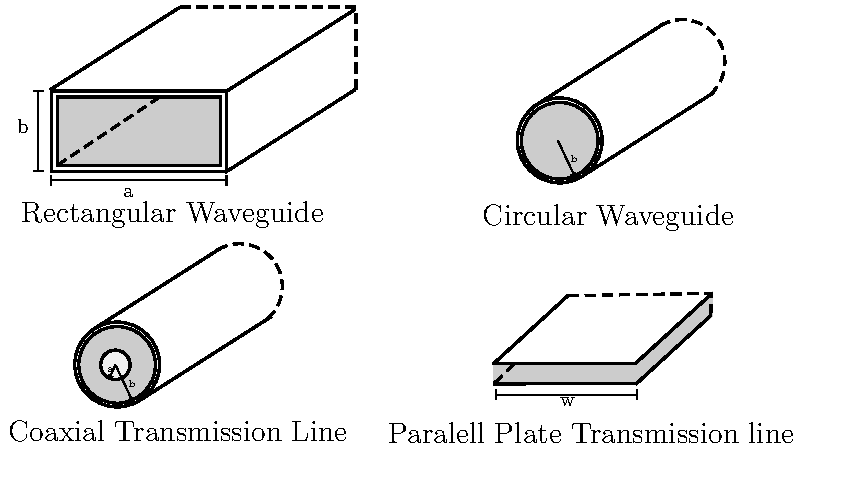
\includegraphics{Figures/Waveguides}
\decoRule
\caption[Waveguide Types]{Types of Waveguides and Transmission Lines}
\label{fig:waveguides}
\end{figure}

\subsubsection{General Waveguide}

Consider a general cross-section of a dielectric surrounded by conductor (can have one more conductor in the dielectric) which continues infinitely along the $z$ axis. We can write down the electric and magnetic fields in the dielectric in phasor domain. We assume that the wave propagates in the $z$-axis and has an $e^{j\omega t}$ dependence.

\begin{equation}
\bar{E}(x,y,z)=[\hat{x}e_x(x,y)+\hat{y}e_y(x,y)+\hat{z}e_z(x,y)]e^{-j\beta z}
\label{eqn:electric field general}
\end{equation}

\begin{equation}
\bar{H}(x,y,z)=[\hat{x}h_x(x,y)+\hat{y}h_y(x,y)+\hat{z}h_z(x,y)]e^{-j\beta z}
\label{eqn:magnetic field general}
\end{equation}

Here $\beta$, the propagation constant, is a real number. $j\beta$ must be replaced with $\gamma=\alpha+j\beta$ if attenuation is also to be considered.

Then, if the dielectric in the waveguide has no charges or currents, we can write Maxwell's equations as

\begin{subequations}
\label{eqn:maxwell curl}
\begin{align}
\nabla \times \bar{E}& =-j\omega \mu \bar{H}
\label{eqn:maxwell electric curl}\\
\nabla \times \bar{H}& =j\omega \epsilon \bar{E}
\label{eqn:maxwell magnetic curl}
\end{align}
\end{subequations}
Taking the curl of \ref{eqn:maxwell electric curl} gives
\begin{equation}
\nabla \times \nabla \times \bar{E}=-j\omega\mu \nabla \times \bar{H}=\omega^2 \mu\epsilon \bar{E}
\end{equation}
Using the vector identity $\nabla\times\nabla\times\bar{A}=\nabla(\nabla .\bar{A})-\nabla^2 \bar{A}$ and $\nabla .\bar{E}=0$ for a region with no sources ($\rho=0$) we get
\begin{equation}
\nabla^2 \bar{E}+\omega^2\mu\epsilon\bar{E}=0
\end{equation}

Similarly, we can also take the curl of \ref{eqn:maxwell magnetic curl} to get
\begin{equation}
\nabla^2 \bar{H}+\omega^2\mu\epsilon\bar{H}=0
\end{equation}

For a $z$ dependence of $e^{-j\beta z}$, $E_z$ and $H_z$ can be written as
\begin{equation}
\left(\frac{\partial^2}{\partial x^2}+\frac{\partial^2}{\partial y^2}+k^2-\beta^2\right)E_z=0
\label{eqn:diff Ez}
\end{equation}
\begin{equation}
\left(\frac{\partial^2}{\partial x^2}+\frac{\partial^2}{\partial y^2}+k^2-\beta^2\right)H_z=0
\label{eqn:diff Hz}
\end{equation}
since $\frac{\partial^2}{\partial z^2}\left(Ae^{-j\beta z}\right)=-\beta Ae^{-j\beta z}$.
Let us define $k_c^2=k^2-\beta^2$ for convenience.

After writing down the 6 equations that arise from \ref{eqn:maxwell curl} and eliminating variables, we can write $E_x$, $E_y$, $H_x$, $H_y$ in terms of $E_z$ and $H_z$ as follows

\begin{subequations}
\label{eqn:general fields}
\begin{align}
E_x& =\frac{-j}{k_c^2}\left(\beta\frac{\partial E_z}{\partial x} + \omega\mu\frac{\partial H_z}{\partial y}\right)
\label{eqn:Ex}
\\
E_y& =\frac{j}{k_c^2}\left(-\beta\frac{\partial E_z}{\partial y}+ \omega\mu\frac{\partial H_z}{\partial x}\right)
\label{eqn:Ey}
\\
H_x& =\frac{j}{k_c^2}\left(\omega\epsilon\frac{\partial E_z}{\partial y}-\beta\frac{\partial H_z}{\partial x}\right)
\label{eqn:Hx}
\\
H_y& =\frac{-j}{k_c^2}\left(\omega\epsilon\frac{\partial E_z}{\partial x}+\beta\frac{\partial H_z}{\partial y}\right)
\label{eqn:Hy}
\end{align}
\end{subequations}
where
\begin{equation}
k_c^2=k^2-\beta^2
\label{eqn:kc definition}
\end{equation}
\begin{equation}
k=\omega \sqrt{\mu\epsilon}=2\pi/\lambda
\label{eqn:k=2pi/lambda}
\end{equation}

These equations (\ref{eqn:diff Ez}, \ref{eqn:diff Hz} and \ref{eqn:general fields}) can be used for any waveguide. There are three types of waves that are possible in waveguides: Transverse Electric and Magnetic mode (TEM), Transverse Electric mode (TE) and Transverse Magnetic mode (TM).

\begin{enumerate}
\item \textbf{TEM modes}

In this mode $E_z=H_z=0$, meaning there are only transverse fields.
\item \textbf{TE modes}

In this mode $E_z=0$, meaning there are only transverse electric fields.
\item \textbf{TM modes}

In this mode $H_z=0$, meaning there are only transverse magnetic fields.
\end{enumerate}

\subsubsection{Rectangular Waveguide}

Let us now concentrate on the fields in a rectangular waveguide. It can be shown that in the TEM mode, fields in the dielectric follow the same rules as electrostatics \cite{Pozar2009}. In a single conductor waveguide like the rectangular waveguide, the electrostatic potential is zero (or constant) which means that $E=0$ and $H=0$. This means we can only have TE and TM modes in the rectangular waveguide (or any single conductor waveguide).

\begin{enumerate}
\item \textbf{TE modes}

Equation \ref{eqn:diff Hz} has been rewritten below with $k^2-\beta^2$ replaced with $k_c$ and divided by $e^{-j\beta z}$.
\begin{equation}
\left(\frac{\partial^2}{\partial x^2}+\frac{\partial^2}{\partial y^2}+k_c^2\right)h_z=0
\label{eqn:hz diff}
\end{equation}
Here, $H_z(x,y,z)=h_z(x,y)e^{-j\beta z}$.

We can solve \ref{eqn:hz diff} using separation of variables. We assume
\begin{equation}
h_z(x,y)=F(x)G(y)
\end{equation}
Substituting this into \ref{eqn:hz diff} gives
\begin{equation}
\frac{1}{F}\frac{d^2F}{dx^2}+\frac{1}{G}\frac{d^2G}{dy^2}+k_c^2=0
\end{equation}
Now, since each term is independent of each other, each term must be a constant. We define the first term to be $k_x^2$ and the second term to be $k_y^2$ to get 
\begin{equation}
k_x^2+k_y^2+k_c^2=0
\end{equation}
Then we get 2 ordinary differential equations
\begin{subequations}
\label{eqn:separation}
\begin{align}
\frac{d^2F}{dx^2}+k_xF& =0\\
\frac{d^2G}{dy^2}+k_yG& =0
\end{align}
\end{subequations}
The general solution to \ref{eqn:separation} is
\begin{subequations}
\begin{align}
F& =A\cos(k_xx)+B\sin(k_xx)\\
G& =C\cos(k_yy)+D\sin(k_yy)
\end{align}
\end{subequations}
Which gives
\begin{equation}
h_z =(A\cos(k_xx)+B\sin(k_xx))(C\cos(k_yy)+D\sin(k_yy))
\label{eqn:hz general}
\end{equation}

Since the boundary conditions we have are that the tangential electric field at the conductor is zero, i.e.
\begin{subequations}
\begin{align}
e_x(x,y)& =0 & \text{ at } y=0 \text{ and } y=b
\label{eqn:ex boundary}\\
e_y(x,y)& =0 & \text{ at } x=0 \text{ and } x=a
\label{eqn:ey boundary}
\end{align}
\end{subequations}

Substituting $E_z=0$ in \ref{eqn:general fields}, we get
\begin{subequations}
\label{eqn:TE transverse diff}
\begin{align}
E_x& =\frac{-j\omega\mu}{k_c^2}\frac{\partial H_z}{\partial y}\\
E_y& =\frac{-j\omega\mu}{k_c^2}\frac{\partial H_z}{\partial x}\\
H_x& =\frac{-j\beta}{k_c^2}\frac{\partial H_z}{\partial x}\\
H_y& =\frac{-j\beta}{k_c^2}\frac{\partial H_z}{\partial y}
\end{align}
\end{subequations}

Now substituting $h_z(x,y)$ from \ref{eqn:hz general} we get the following electric fields
\begin{subequations}
\begin{align}
e_x& =\frac{-j\omega\mu}{k_c^2}k_y(A\cos(k_xx)+B\sin(k_xx))(-C\sin(k_yy)+D\cos(k_yy))\\
e_y& =\frac{j\omega\mu}{k_c^2}k_x(-A\sin(k_xx)+B\cos(k_xx))(C\cos(k_yy)+D\sin(k_yy))
\end{align}
\end{subequations}
Now applying the boundary conditions,\\
from \ref{eqn:ex boundary} we get $D=0$ and $k_y=n\pi/b$ for $n={0,1,2\ldots}$,\\
and from \ref{eqn:ey boundary} we get $B=0$ and $k_x=m\pi/a$ for $m={0,1,2\ldots}$.\\
From this we know the propagation constant is
\begin{equation}
\beta = \sqrt{k^2-k_c^2}=\sqrt{k^2-\left(\frac{m\pi}{a}\right)^2-\left(\frac{n\pi}{b}\right)^2}
\end{equation}
Since $\beta$ is real, we now have a cut-off frequency for which $k^2>k_c^2$. This means that if $a>b$, there will be a range of frequencies for which $TE_{mn}=TE_{10}$ will have propagation but $TE_{01}$ will not.

The final solution for $H_z$ is
\begin{equation}
H_z(x,y,z)=A_{mn}\cos\left(\frac{m\pi x}{a}\right)\cos\left(\frac{n\pi y}{b}\right)e^{-j\beta z}
\label{Hz final}
\end{equation}
where $A_{mn}=AC$.

Now we can find $E_x, E_y, H_x$ and $H_y$ using \ref{eqn:TE transverse diff}
\begin{subequations}
\label{eqn:TE transverse fields}
\begin{align}
E_x(x,y,z)& =\frac{j\omega\mu n\pi}{k_c^2b}A_{mn}\cos\left(\frac{m\pi x}{a}\right)\sin\left(\frac{n\pi y}{b}\right)e^{-j\beta z}\\
E_y(x,y,z)& =\frac{-j\omega\mu m\pi}{k_c^2a}A_{mn}\sin\left(\frac{m\pi x}{a}\right)\cos\left(\frac{n\pi y}{b}\right)e^{-j\beta z}\\
H_x(x,y,z)& =\frac{j\beta m\pi}{k_c^2a}A_{mn}\sin\left(\frac{m\pi x}{a}\right)\cos\left(\frac{n\pi y}{b}\right)e^{-j\beta z}\\
H_y(x,y,z)& =\frac{j\beta n\pi}{k_c^2b}A_{mn}\cos\left(\frac{m\pi x}{a}\right)\sin\left(\frac{n\pi y}{b}\right)e^{-j\beta z}
\end{align}
\end{subequations}

These equations are only for a wave propagating in one direction. The total electric field well have another term for the fields with a different constant. We can replace $A_{mn}$ with $A_{mn}^+$ (for $+z$ direction propagation) and $A_{mn}^-$ (for $-z$ direction propagation). Then the transverse fields for each mode ($m,n$) would take the form
\begin{subequations}
\begin{align}
\bar{E}_t(x,y,z)& =[\hat{x}e_x(x,y)+\hat{y}e_y(x,y)](A^+e^{-j\beta z}+A^-e^{+j\beta z})\\
\bar{H}_t(x,y,z)& =[\hat{x}h_x(x,y)+\hat{y}h_y(x,y)](A^+e^{-j\beta z}-A^-e^{+j\beta z})
\end{align}
\end{subequations}
The negative sign for $A^-$ in the magnetic field is to ensure that the direction of propagation given by $\bar{E}_t\times\bar{H}_t$ is opposite.

\item \textbf{TM modes}

The TM modes can be derived in exactly the same way except that the boundary conditions will apply directly to $E_z$ this time.

The fields for the TM modes are
\begin{subequations}
\begin{align}
E_z(x,y,z)& =B_{mn}\sin\left(\frac{m\pi x}{a}\right)\sin\left(\frac{n\pi y}{b}\right)e^{-j\beta z}\\
E_x(x,y,z)& =\frac{-j\beta m\pi}{k_c^2a}B_{mn}\cos\left(\frac{m\pi x}{a}\right)\sin\left(\frac{n\pi y}{b}\right)e^{-j\beta z}\\
E_y(x,y,z)& =\frac{-j\beta n\pi}{k_c^2b}B_{mn}\sin\left(\frac{m\pi x}{a}\right)\cos\left(\frac{n\pi y}{b}\right)e^{-j\beta z}\\
H_x(x,y,z)& =\frac{j\omega\epsilon n\pi}{k_c^2b}B_{mn}\sin\left(\frac{m\pi x}{a}\right)\cos\left(\frac{n\pi y}{b}\right)e^{-j\beta z}\\
H_y(x,y,z)& =\frac{-j\omega
\epsilon m\pi}{k_c^2a}B_{mn}\cos\left(\frac{m\pi x}{a}\right)\sin\left(\frac{n\pi y}{b}\right)e^{-j\beta z}
\end{align}
\end{subequations}

Notice that if $m$ or $n$ is zero, then the fields all go to zero. So there is no $TM_{10}$ or $TM_{01}$ mode.

The propagation constant $\beta$ is
\begin{equation}
\beta = \sqrt{k^2-k_c^2}=\sqrt{k^2-\left(\frac{m\pi}{a}\right)^2-\left(\frac{n\pi}{b}\right)^2}
\end{equation}

This means the cut-off frequencies are the same for the TE and TM modes. Now we can see that there is a range of frequencies where only the $TE_{10}$ mode will propagate. This feature of waveguides is used extensively to avoid complications of other modes interfering with the signal.
\end{enumerate}


%-----------------------------------
%	SUBSECTION 2
%-----------------------------------

\subsection{Rectangular Waveguide Resonators}

Now that we know what modes and what frequencies can propagate in a rectangular waveguide, we can convert the waveguide into a resonator by walling the 2 infinitely open faces with conducting surfaces to make a cuboid filled with dielectric. This structure is often called a rectangular cavity.\\

We can use the equations we derived in the previous section for fields and the propagation constant to see what effects the new conducting walls will have.

We can start by writing down the transverse electric field ($E_t = \hat{x}E_x+\hat{y}E_y$)
\begin{equation}
\bar{E}_t=\bar{e}(x,y)(A^+e^{-j\beta z}+A^-e^{+j\beta z})
\label{eqn:Et start}
\end{equation}
where $\bar{e}(x,y)$ is the variation in the transverse fields.
\begin{equation}
\beta = \sqrt{k^2-\left(\frac{m \pi}{a}\right)^2-\left(\frac{n \pi}{b}\right)^2}
\end{equation}

The new boundary conditions added now are that $E_t=0$ at the 2 new walls, $z=0$ and $z=d$.\\
For $z=0$, \ref{eqn:Et start} gives 
\begin{equation}
A^+=-A^-
\end{equation}.\\
For $z=d$, \ref{eqn:Et start} gives
\begin{equation}
-\bar{e}(x,y)A^+2j\sin(\beta_{mn}d)=0
\end{equation}
The solution to this equation (other than $A^+=0$) is
\begin{equation}
\beta_{mn}=\frac{l\pi}{d} \text{ where } l=1,2,3\ldots
\end{equation}
This means that, given a frequency, propagation (or in this case resonance) occurs only for particular lengths. $\beta^2=k^2-k_c^2$ can be rearranged to get
\begin{equation}
k_{mnl}=\sqrt{\left(\frac{m \pi}{a}\right)^2+\left(\frac{n \pi}{b}\right)^2+\left(\frac{l \pi}{d}\right)^2}
\end{equation}
The resonant frequency is given by
\begin{equation}
f_{mnl}=\frac{ck_{mnl}}{2\pi\sqrt{\mu_r\epsilon_r}}=\frac{c}{2\pi\sqrt{\mu_r\epsilon_r}}\sqrt{\left(\frac{m \pi}{a}\right)^2+\left(\frac{n \pi}{b}\right)^2+\left(\frac{l \pi}{d}\right)^2}
\end{equation}

Now let us restrict ourselves to the $TE_{10l}$ mode of the resonator. Since $A^-=-A^+$, the fields for this mode are
\begin{subequations}
\label{eqn:TE10l fields}
\begin{align}
E_y(x,y,z)& =A^+\sin\left(\frac{\pi x}{a}\right)(e^{-j\beta z}-e^{+j\beta z})\\
H_x(x,y,z)& =\frac{-A^+}{Z_{TE}}\sin\left(\frac{\pi x}{a}\right)(e^{-j\beta z}+e^{+j\beta z})\\
H_z(x,y,z)& =\frac{j\pi A^+}{k\eta a}\cos\left(\frac{\pi x}{a}\right)(e^{-j\beta z}-e^{+j\beta z})
\end{align}
\end{subequations}
where
\begin{subequations}
\begin{align*}
A^+& =\frac{-j\omega\mu m\pi}{k_c^2a}\\
Z_{TE}& =\frac{\omega\mu}{\beta}& 
k& =\omega\sqrt{\mu\epsilon}\\
k_c^2& =\sqrt{\frac{\pi}{a}}& 
\eta& =\sqrt{\frac{\mu}{\epsilon}}
\end{align*}
\end{subequations}

Using $-2jA^+=E_0$, we can simplify the above equations to
\begin{subequations}
\begin{align}
E_y(x,y,z)& =E_0\sin\left(\frac{\pi x}{a}\right)\sin\left(\frac{l\pi z}{d}\right)\\
H_x(x,y,z)& =\frac{-jE_0}{Z_{TE}}\sin\left(\frac{\pi x}{a}\right)\cos\left(\frac{l\pi z}{d}\right)\\
H_z(x,y,z)& =\frac{j\pi E_0}{k\eta a}\cos\left(\frac{\pi x}{a}\right)\sin\left(\frac{l\pi z}{d}\right)
\end{align}
\end{subequations}

We can now calculate the \textit{quality factor} $Q$ by calculating the energy stored and power lost in the resonator.
The stored electric energy is, from \cite{Pozar2009}
\begin{equation}
W_e=\frac{\epsilon}{4}\int_V E_yE_y^*dv = \frac{\epsilon abd}{16}E_0^2
\end{equation}
and the stored magnetic energy is
\begin{align}
\begin{split}
W_m&=\frac{\mu}{4}\int_V (H_xH_x^*+H_zH_z^*)dv\\
&= \frac{\mu abd}{16}E_0^2\left(\frac{1}{Z_{TE}^2}+\frac{\pi^2}{k^2\eta^2a^2}\right)\\
&=\frac{\mu abd}{16}E_0^2\left(\frac{\beta^2+(\pi/a)^2}{k^2\eta^2}\right)\\
&=\frac{\mu abd}{16}E_0^2\left(\frac{1}{\eta^2}\right)\\
&=\frac{\epsilon abd}{16}E_0^2
\end{split}
\end{align}
Note that $W_e=W_m$ at resonance.

The power lost by the conducting walls is
\begin{equation}
P_c=\frac{R_s}{2}\int_{walls} |H_t|^2ds
\end{equation}
where $R_s=\sqrt{\omega\mu_0/(2\sigma)}$ is the surface resistivity and $H_t$ is the tangential magnetic field at the walls. This gives
\begin{equation}
P_c=\frac{R_sE_0^2\lambda^2}{8\eta^2}\left(\frac{l^2ab}{d^2}+\frac{bd}{a^2}+\frac{l^2a}{2d}+\frac{d}{2a}\right)
\end{equation}

The power dissipated from the lossy dielectric with $\epsilon = \epsilon'-j\epsilon''$ is
\begin{equation}
P_d = \frac{1}{2}\int_V\bar{J}.\bar{E}=\frac{\omega\epsilon''}{2}\int_V|\bar{E}|^2dv=\frac{abd\omega\epsilon''|E_0|^2}{8}
\end{equation}

The quality factor $Q$ is defined as
\begin{align}
\begin{split}
Q&=\omega\frac{\text{average energy stored}}{\text{average power loss}}\\
&=\omega\frac{W_e+W_m}{P_{loss}}\\
&=\omega\frac{2W_e}{P_c+P_d}
\end{split}
\end{align}

\subsection{Coupling to an External Circuit}

A resonator is useless if we cannot communicate with it in some way. There are many ways of interacting with a resonator. In the experiments to follow, the rectangular cavity resonator will be coupled to and external circuit through a probe of height $h$ inserted at the $y=0$ wall at $x=a/4$ and $z=0$. A figure of the probe inserted in the rectangular cavity is shown in Fig.\ref{fig:Probe}.

\begin{figure}
\centering
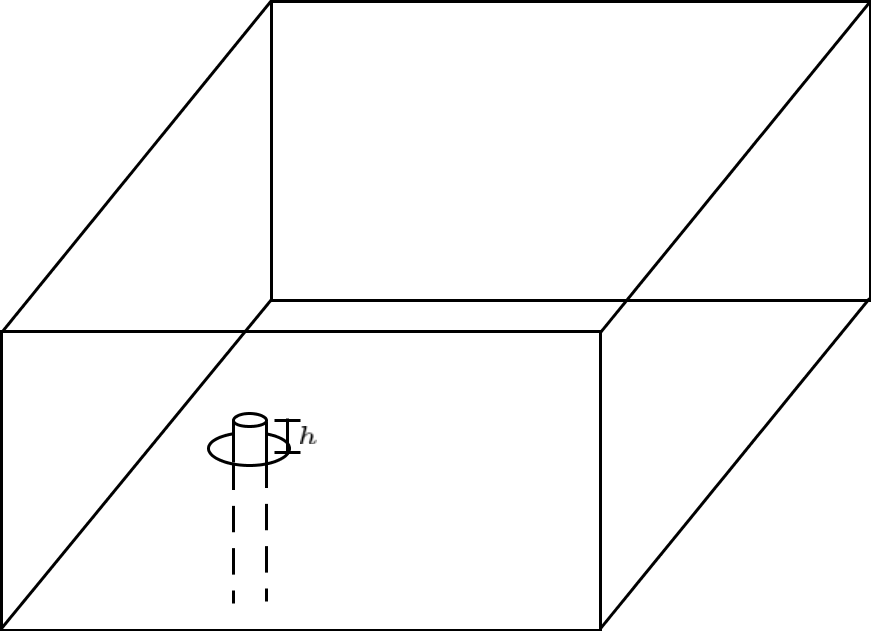
\includegraphics[width=250px]{Figures/probe}
\decoRule
\caption[Probe in resonator]{The probe is inserted up to a height $h$ into the cavity. The other end of the probe is a coaxial cable whose outer terminal is connected to the cavity.}
\label{fig:Probe}
\end{figure}

The equivalent circuit, shown in Fig.\ref{fig:external circuit} for this setup would be a paralell RLC circuit capacitively coupled to the measurement device, which in this case is a VNA (Vector Network Analyzer).

\begin{figure}
\centering
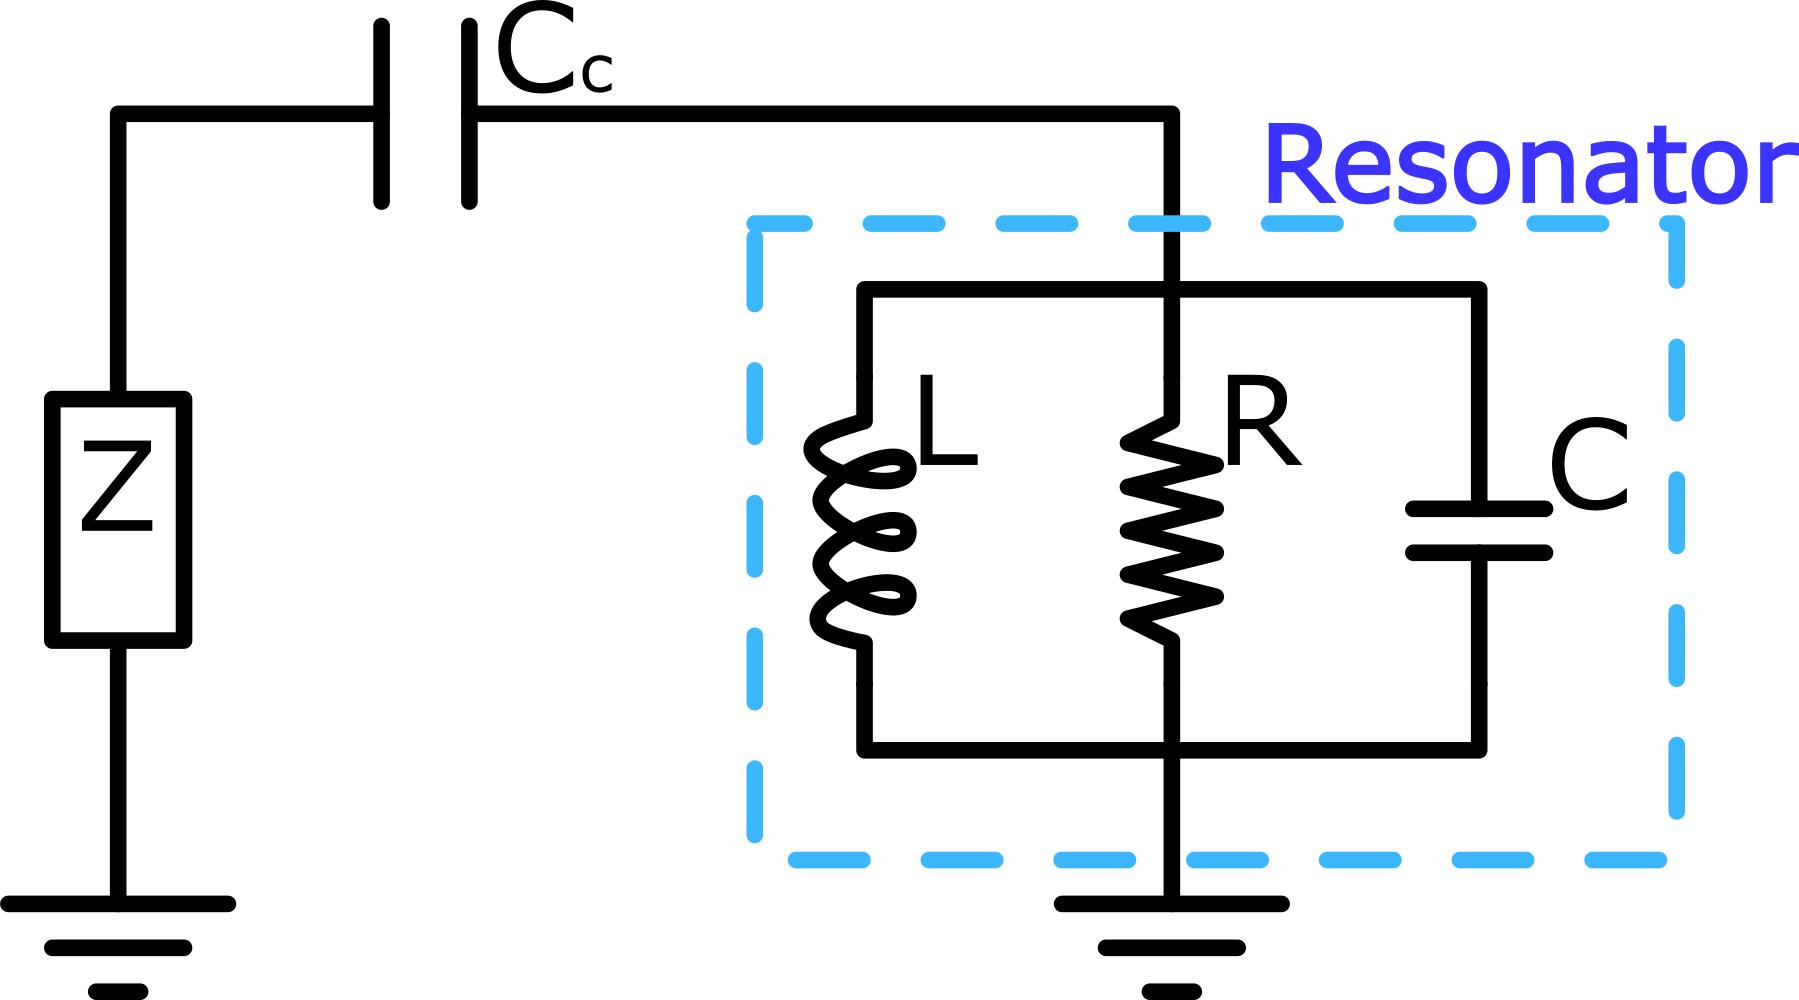
\includegraphics[width=250px]{Figures/external.png}
\decoRule
\caption[External coupling circuit]{The equivalent circuit for the resonator is a parallel RLC circuit.The external losses are in the external inpedence Z of the meaasurement device. The energy in the resonator leaks to the external circuit at a rate $\kappa_e\propto 1/C_c$. The internal losses are due to the resistance R. The rate of instrinsic energy loss in the resonator is $\kappa_i = \kappa - \kappa_e$ where $\kappa$ is the FWHM of the $S_{11}$ response of the resonator.}
\label{fig:external circuit}
\end{figure}

\section{Experiment}

The rectangular cavity used for the experiment is made of aluminium and is shown in Fig.\ref{fig:cavity}.

\begin{figure}
\centering
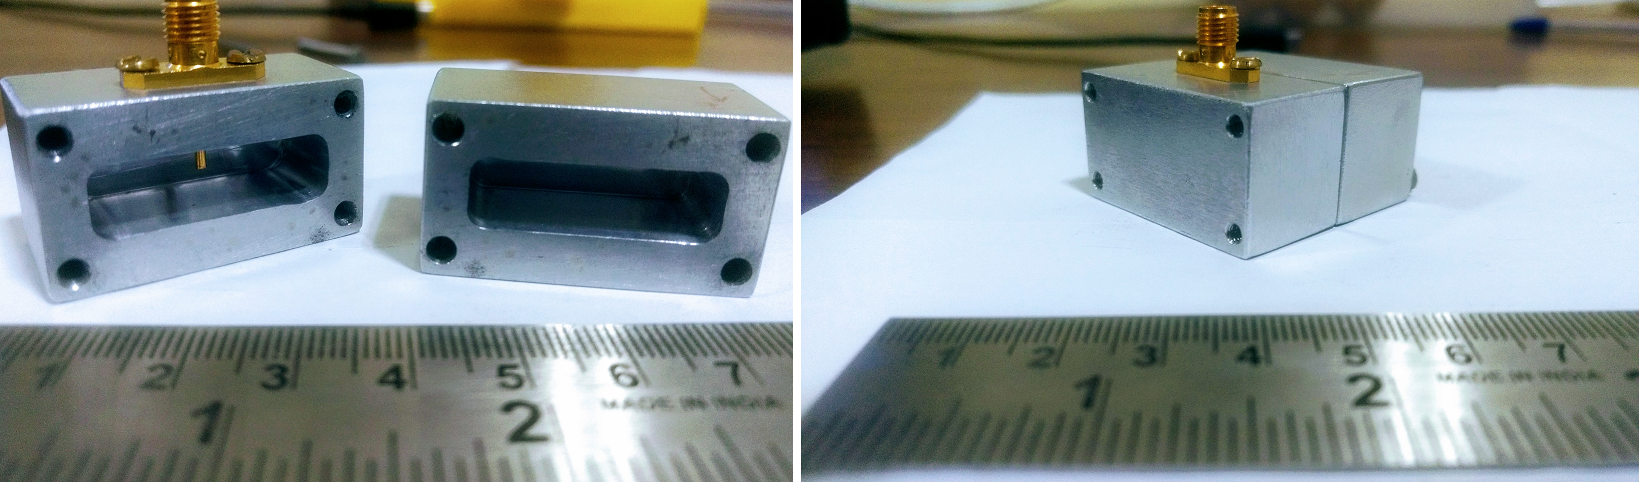
\includegraphics[width=350px]{Figures/cavity.png}
\decoRule
\caption[Aluminium Cavity]{The Aluminium cavity used to make measurements. The dimensions of the hollow in the assembled cavity are $36\times 27\times 8\SI{}{\milli\meter}$. The lengths of the connector pin referred to by Fig.\ref{fig:diff lengths} includes the wall of the cavity.}
\label{fig:cavity}
\end{figure}

The $S_{11}$ parameter is the ratio of the voltage detected to voltage sent into the cavity. It is a complex number with information about the amplitude and phase. It it measured by sending a known signal of a particular frequency with a set amplitude and phase, and detecting the amplitude and phase of the reflected signal after passing through the cavity at the same frequency. A VNA is used to sweep the frequency of the input signal and record the amplitude and phase of the signal returned at the same frequency. The schematic of the circuit used to make measurements at $20mK$ is shown in Fig.\ref{fig:circuit with fridge}. The actual setup of the dilution refrigerator is shown in Fig.\ref{fig:real fridge}.

\begin{figure}
\centering
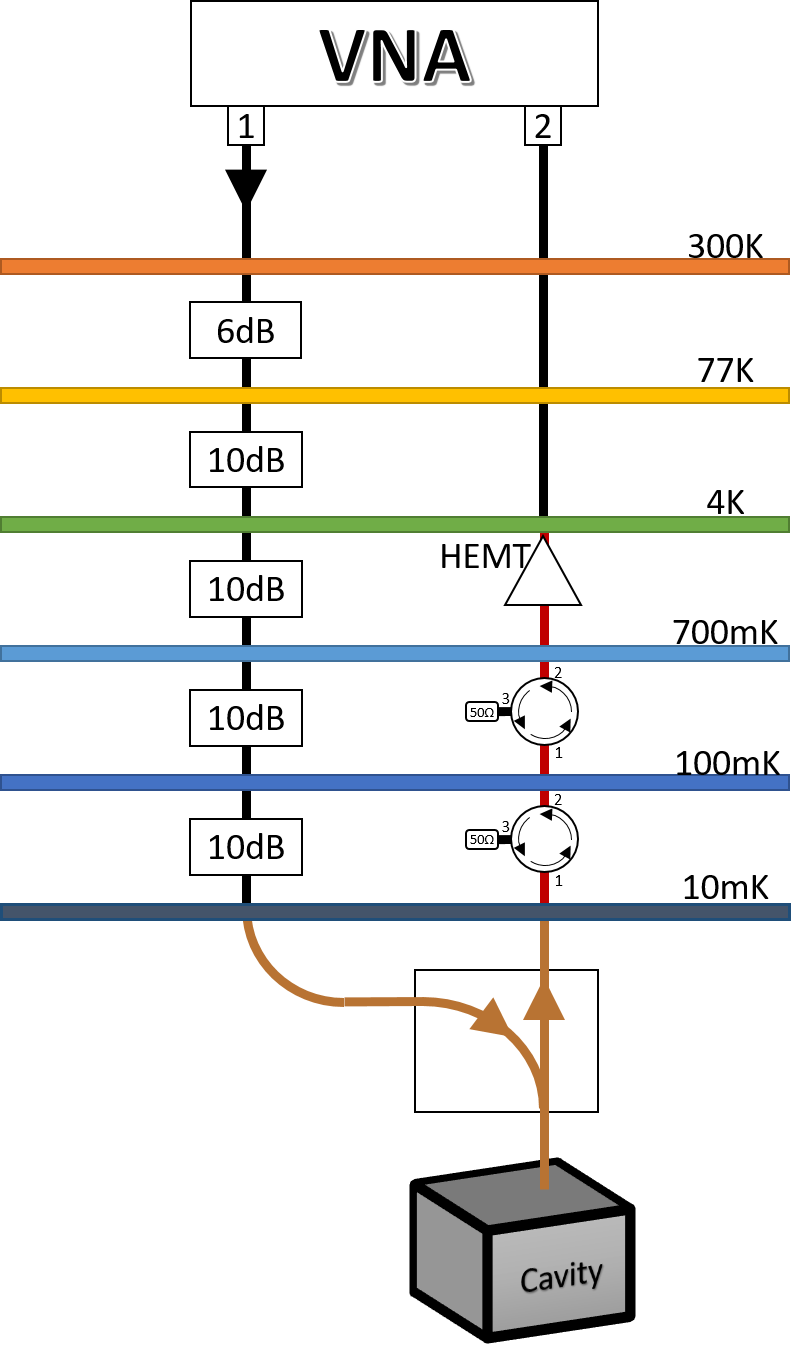
\includegraphics[width=350px]{Figures/circuit.png}
\decoRule
\caption[External Circuit]{The measurement setup for $20mK$ measurements. The input signal is sent from port 1 of the VNA. There are attenuators of appropriate values in between the plates. At the base plate, the input goes into a directional coupler which adds another 20dB attenuation. The output from the cavity is directed towards a HEMT amplifier which is connected to port 2 of the VNA.}
\label{fig:circuit with fridge}
\end{figure}

\begin{figure}
\centering
\includegraphics[width=350px]{Figures/dil_fridge.jpg}
\decoRule
\caption[Dilution Refrigerator]{The Dilution Refrigerator.}
\label{fig:real fridge}
\end{figure}

The $S_{11}$ response for a microwave resonator is given by \cite{Aspelmeyer2014}
\begin{equation}
S_{11}(\omega) = 1-\frac{\kappa_e}{\kappa/2+j(\omega-\omega_0)}
\label{eqn:s11 sym}
\end{equation}
where\\
$\omega_0$ is the resonant frequency of the cavity,\\
$\kappa = \Delta\omega$ is the FWHM of the resonance peak which represents total losses,\\
$\kappa_e$ is the part of $\kappa$ which represents the losses to the external circuit through the capacitor $C_c$.\\
The quality factor can be calculated using $Q = \omega_0/\text{FWHM}$. The internal, external and total quality factors can be calculated using
\begin{align}
Q_{total} &= \frac{\omega_0}{\kappa}\\
Q_{external} &= \frac{\omega_0}{\kappa_e}\\
Q_{internal} &= \left(\frac{1}{Q_{total}}-\frac{1}{Q_{external}}\right)^{-1}\\
\end{align}

The $S_{11}$ response of the cavity is asymmetrical, as shown in Fig. \ref{fig:cavity response}, due to the finite cable length and finite isolation of the directional coupler.
\begin{itemize}
\item The effect of the finite cable length is an added frequency dependent phase factor $\text{exp}(2j\omega l/v_p)$ where $l$ is the cable length and $v_p=c/\sqrt{\epsilon_r}$ is the phase velocity. The '$2$' in the expression is because the cable length is traversed twice.\\
This factor is multiplied to the original expression for $S_{11}$ in \ref{eqn:s11 sym}.
\item The effect of the finite isolation of the directional coupler is modelled by considering a part of the signal as a complex background ($\alpha_i e^{j\phi}$) and the rest of the signal ($(1-\alpha_i)S_{11}$) as the $S_{11}$ response.
\end{itemize}
So the final function used to fit the data from Fig.\ref{fig:circuit with fridge} and get the parameters $\omega_0$,$\kappa$ and $\kappa$ is
\begin{equation}
S_{11}(\omega) = \alpha_i e^{j\phi}+(1-\alpha_i)\left(1-\frac{\kappa_e}{\kappa/2+j(\omega-\omega_0)}\right)e^{2j\omega l/v_p}
\end{equation}

\begin{figure}
\centering
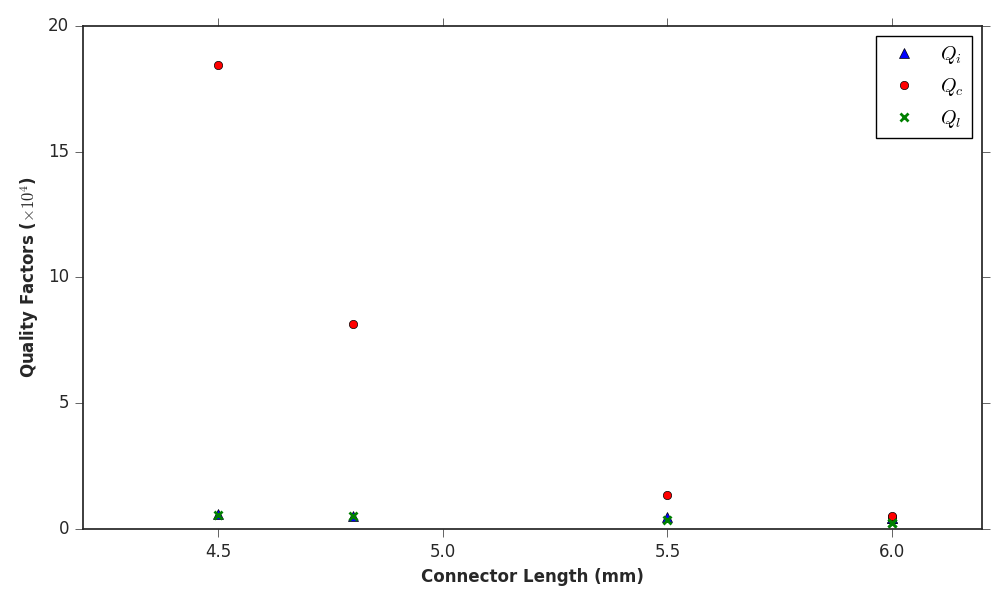
\includegraphics[width=\linewidth]{Figures/diff_lengths.png}
\decoRule
\caption[Quality Factors for different pin lengths]{Quality factors for different pin lengths. $Q_i$ is the internal Quality, $Q_c$ is the external Quality, and $Q_t$ is the total Quality. The coupling Quality Factor $Q_c$ is increasing with decreasing pin lengths.}
\label{fig:diff lengths}
\end{figure}

The $S_{11}$ measurement was performed for different pin lengths\footnote{The lengths of the connector pin referred to here includes the wall of the cavity. So, the actual length of the connector pin that is in the cavity is $\SI{5}{\milli\meter}$ lesser than the given length.} inserted into the cavity at room temperature. This was done in order to tune the coupling quality factor $Q_c$ such that the internal quality factor $Q_i$ would be equal to $Q_c$ once the cavity is cooled to $\SI{20}{\milli]kelvin}$, leading to a critically coupled system.

The quality factors obtained from this measurement are shown in Fig.\ref{fig:diff lengths}. The coupling Quality Factor $Q_c$ increases with decreasing pin length, while the internal Quality Factor remains the same.

The same measurement is made by using a constant pin length of $4.5 mm$, but this time at a temperature of $20mK$. The internal quality factor is larger than the coupling quality factor at this temperature mainly because aluminium is superconducting below $1.1K$. Fig.\ref{fig:cold qualities} shows a plot of $Q_i$, $Q_c$ and $Q_t$ as a function of the average number of photons in the cavity. A sample plot of amplitude and phase data for a power of -35dBm is shown in Fig.\ref{fig:fit}. The coupling Quality Factor $Q_c$ remains the same, suggesting that it does not depend on the number of photons in the cavity. The internal Quality Factor has an increasing trend. This can be explained using Two-Level Systems in the material which get saturated to their excited states at higher photon numbers\cite{Gao2007}.

\begin{figure}
\centering
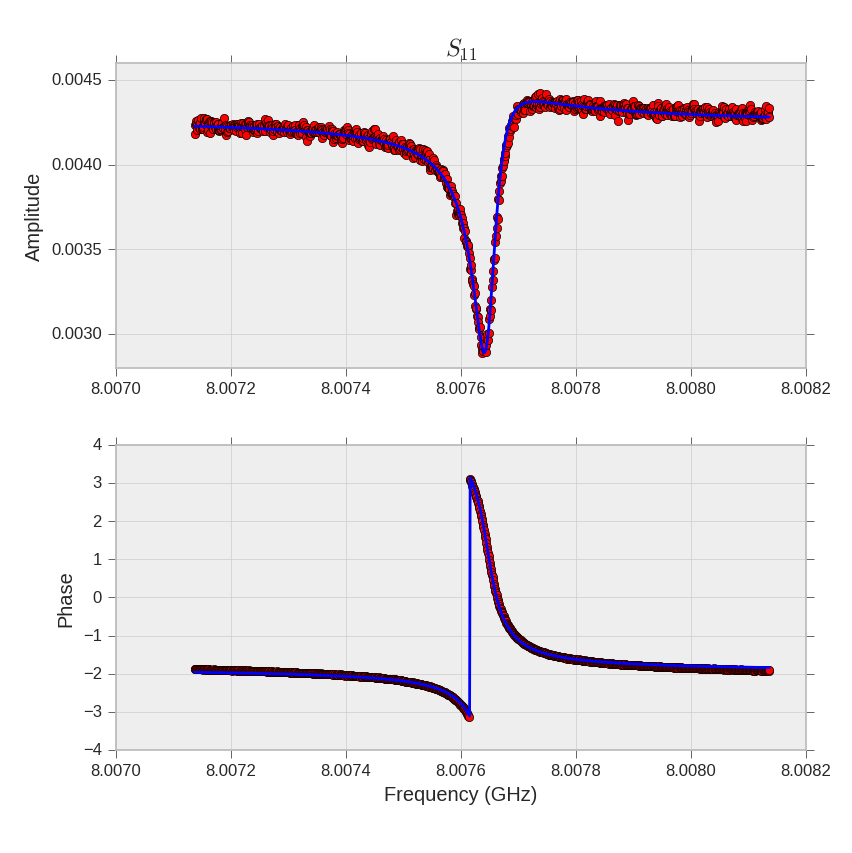
\includegraphics[width=300px]{Figures/s11fit.png}
\decoRule
\caption[Sample $S_{11}$ fit]{A sample of data and fit of $S_{11}$ at 20mK for a power of -35dBm. The red dots are the data from the VNA, and the blue line is the fit.}
\label{fig:fit}
%\end{figure}

%\begin{figure}
\centering
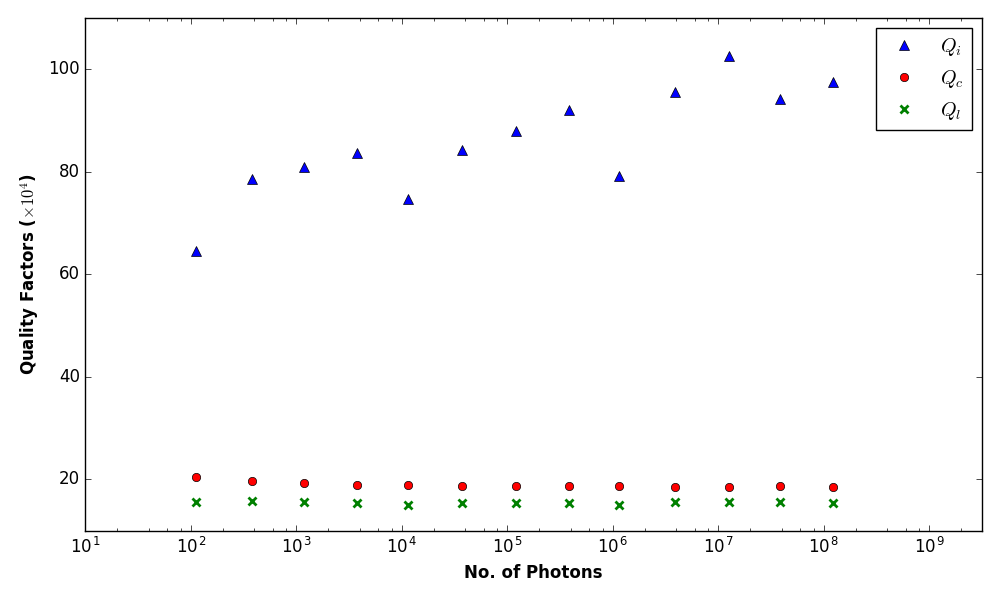
\includegraphics[width=\linewidth]{Figures/cold_qualities.png}
\decoRule
\caption[Quality Factors for different powers at low temperature]{Quality factors for different powers at low temperature. $Q_i$ is the internal Quality, $Q_c$ is the external Quality, and $Q_t$ is the total Quality.}
\label{fig:cold qualities}
\end{figure} 
% Chapter Template

\chapter{Superconducting Qubit Theory} % Main chapter title

\label{Chapter3} % Change X to a consecutive number; for referencing this chapter elsewhere, use \ref{ChapterX}

%----------------------------------------------------------------------------------------
%	SECTION 1
%----------------------------------------------------------------------------------------
\section{Classical LC oscillator}

%------------ FILL THE LC OSCILLATOR FIGURE -----------
\begin{figure}
\centering
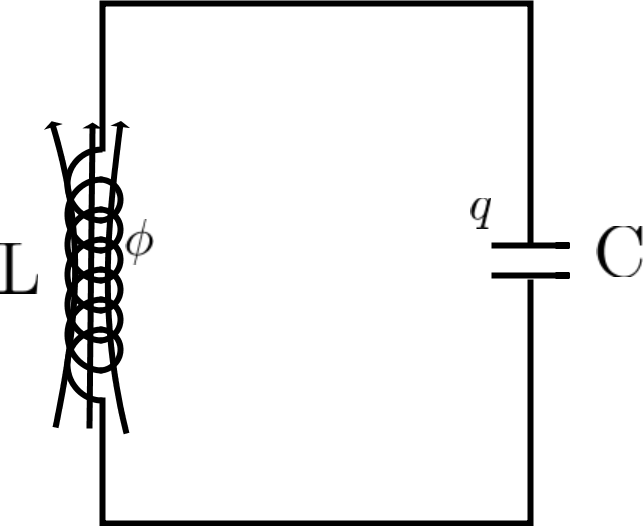
\includegraphics[width=150pt]{Figures/LC_oscillator}
\decoRule
\caption[LC oscillator]{LC oscillator circuit}
\label{fig:LC oscillator}
\end{figure}

The LC oscillator, shown in Fig.\ref{fig:LC oscillator}, when treated classically has a charge $q$ on the capacitor, and a flux $\phi$ in the inductor. The flux is related to the charge via the inductance as $\phi=L\dfrac{dq}{dt}$. The Hamiltonian for this circuit is
\begin{equation}
\mathcal{H}=\frac{q^2}{2C}+\frac{\phi^2}{2L}
\end{equation}

\section{Quantum Electrical Circuits}

\subsection{Quantum LC oscillator}

Observe that the 2 variables involved in the LC oscillator, $q$ and $\phi=L\dfrac{dq}{dt}$, are similar in form to the position and momentum operators in quantum mechanics, $\hat{x}$ and $\hat{p}=-j\hbar\dfrac{\partial}{\partial x}$. Even the Hamiltonian is of the same form.\parencite{Devoret1995}
\begin{equation}
\hat{\mathcal{H}}=\frac{\hat{p}^2}{2m}+\frac{m\omega^2\hat{x}^2}{2}
\end{equation}
Because of this, we can treat this circuit like the simple harmonic oscillator and introduce the annihilation and creation operators to define $\hat{q}$, $\hat{\phi}$ and Hamiltonian operators as
\begin{subequations}
\begin{align}
\hat{\phi}&=\frac{1}{j}\sqrt{\frac{\hbar}{2Z_0}}(a-a^\dag)\\
\hat{q}&=\sqrt{\frac{\hbar Z_0}{2}}(a+a^\dag)\\
\hat{\mathcal{H}}&=\frac{\hbar\omega_0}{2}(a^\dag a+aa^\dag)=\hbar\omega_0\left(a^\dag a + \frac{1}{2}\right)
\label{eqn:harmonic hamiltonian}
\end{align}
\end{subequations}
where
\begin{align*}
[\hat{\phi},\hat{q}]=-j\hbar&&
\omega_0=\frac{1}{\sqrt{LC}}&&
Z_0=\sqrt{\frac{L}{C}}
\end{align*}
$\omega_0$ and $C$ in the LC oscillator is analogous to $\omega$ and $m$ in the harmonic oscillator.

We can write the wave-functions of the energy eigenstates of the LC oscillator as
\begin{equation}
\bra{x}\ket{0}=\psi_0=\left(\frac{C\omega_0}{\pi\hbar}\right)^\frac{1}{4}e^{-\left(\frac{C\omega_0}{2\hbar}\right)x^2}
\end{equation}
This solution can be obtained using $a\ket{0}=0$

The rest of the eigenstates can be obtained by using the creation operator $a^\dag$ since
\begin{equation}
a^\dag\ket{n}=\sqrt{n+1}\ket{n+1}
\end{equation}
which gives
\begin{equation}
\ket{n}=\frac{(a^\dag)^n}{\sqrt{n!}}\ket{0}
\end{equation}
The energy corresponding to these states are
\begin{equation}
E_n=\left(n+\frac{1}{2}\right)\hbar\omega_0
\end{equation}
The general solution to the Schr\"{o}dinger equation $\hat{\mathcal{H}}\ket{\psi}=E\ket{\psi}$ is
\begin{equation}
\ket{\psi}=\sum_nc_n\ket{n}
\end{equation}
The first few energy levels along with the corresponding wavefunctions are shown in Fig.\ref{fig:harmonic oscillator}.

\begin{figure}
\centering
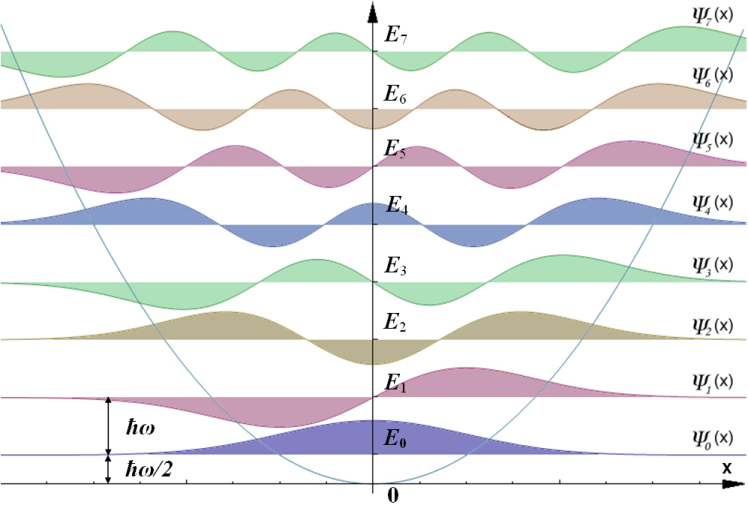
\includegraphics[width=\linewidth]{Figures/harmonic_oscillator}
\decoRule
\caption[Harmonic Oscillator Energy Levels]{The harmonic oscillator potential showing the Energy Levels $E_1,E_2,\ldots$ along with the corresponding wavefunctions $\psi_1,\psi_2,\ldots$. Replacing the position coordinate here with charge would give us the Energy levels for an LC oscillator.Taken from \\© \href{https://pl.wikipedia.org/wiki/Wikipedysta:Tomasz59}{User:Tomasz59} / \href{http://commons.wikimedia.org/}{Wikimedia Commons} / \href{http://creativecommons.org/licenses/by-sa/3.0/}{CC-BY-SA-3.0}}
\label{fig:harmonic oscillator}
\end{figure}

Coherent states of a harmonic oscillator are defined as the eigenstates of the amplitude operator, or annhilation operator $a$, such that
\begin{equation}
a\ket{\alpha} = \alpha\ket{\alpha}
\end{equation}
where $\alpha = |\alpha|e^{j\varphi}$ is a complex number and corresponds to the complex wave amplitude in classical optics. Thus coherent states are wave-like states of the electromagnetic oscillator is a complex number \cite{Glauber1963}.

The coherent state $\ket{\alpha}$ can be represented in terms of the number states $\ket{n}$ as
\begin{equation}
\ket{\alpha} = \sum_{n=0}^\infty \frac{\alpha^n}{\sqrt{n!}}e^{-|\alpha|^2/2}\ket{n}
\label{eqn:glauber expansion}
\end{equation}

\subsection{Nonlinear Harmonic Oscillator}

Note that the energy levels in the Simple Harmonic Oscillator (SHO) or the LC oscillator are equispaced. This means that if we supply a photon of energy $\hbar\omega_0$ to the LC oscillator, we can change the state from any $\ket{n}$ to $\ket{n+1}$, and all photons emitted due to the transition from $\ket{n}$ to $\ket{n-1}$ will have the same energy.

A Nonlinear Harmonic Oscillator is one where the energy levels do not increase linearly. We can create a nonlinear oscillator by adding a perturbation to the Hamiltonian. The new Hamiltonian will be of the form
\begin{equation}
\hat{\mathcal{H}}=\frac{q^2}{2C}+\frac{\phi^2}{2L} +\mathcal{H}'
\end{equation}
where $H'$ is the perturbation term.
The energy levels for this new Hamiltonian can be written in terms of the unperturbed Hamiltonian using perturbation theory as
\begin{equation}
E_n=E_n^{(0)}+\expval{\mathcal{H}'}{n^{(0)}}+\sum_{k\neq n}\frac{\left|\mel{k^{(0)}}{\mathcal{H}'}{n^{(0)}}\right|^2}{E_n^{(0)}-E_k^{(0)}}+\ldots
\end{equation}
where,\\
$E_n$ is the new energy for the $n$th eigenstate,\\
$E_n^{(0)}$ is the energy for the $n$th eigenstate of the unperturbed Hamiltonian,\\
$\expval{\mathcal{H}'}{n^{(0)}}$ is the first order correction to the energy and\\
$\sum_{k\neq n}\frac{\left|\mel{k^{(0)}}{\mathcal{H}'}{n^{(0)}}\right|^2}{E_n^{(0)}-E_k^{(0)}}$ is the second order correction to the energy.

If the perturbation $\mathcal{H}'$ is not a constant (i.e $\mathcal{H}'(n)\neq \mathcal{H}'(m)$ where $n\neq m$), then we can access only the ground state and the first exited state with one frequency of photons. This is because if the particle is in the first excited state, and another photon of the same energy ($E_{10}=E_1-E_0$) is supplied to the system, it will not excite the particle further.

This means that we can selectively access only 2 states. If we can manipulate such a 2 level system and it's interactions, we have a qubit!

\section{The Josephson Junction}

The \JJ is the nonlinear element used in the described experiments due to it's negligible dissipation rate which is essential for working in the quantum regime.\\
The \JJ is made of 2 superconductors coupled by a weak link. In our case the junction is an S-I-S (Superconductor-Insulator-Superconductor) junction as shown in Fig.\ref{fig:SISJJ}.

\begin{figure}
\centering
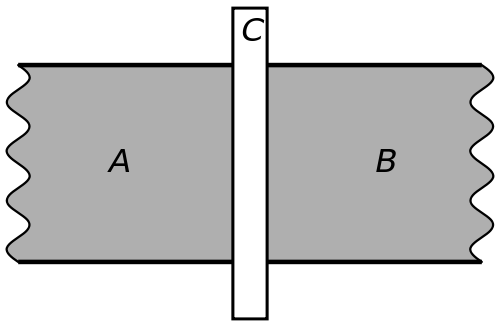
\includegraphics[width=\linewidth]{Figures/SISJJ}
\decoRule
\caption[Josephson Junction]{Simple geometric structure of a \JJ with A and B being superconducting regions and C being the thin insulating layer.}
\label{fig:SISJJ}
\end{figure}

Electrons in a normal metal behave like fermions. But at very low temperatures, they form cooper pairs that act like bosons. Nearly all the bosons will be at the lowest energy in exactly the same state \cite{Feynman1966}. This means that the superconductor will have a macroscopic wavefunction with a single homogeneous amplitude and phase.

In the \JJ, there are two superconductors, and so we can define 2 amplitudes and 2 phases corresponding to each superconductor.
\begin{align*}
\psi_1&=\sqrt{\rho_1}e^{j\theta_1}\\
\psi_2&=\sqrt{\rho_2}e^{j\theta_2}
\end{align*}
Then, the current and voltage characteristics are given by \cite{Harmans1997}
\begin{align}
I_s&=I_0\sin\delta
\label{eqn:JJ current}\\
V&=\frac{\Phi_0}{2\pi}\dot{\delta}
\label{eqn:JJ voltage}
\end{align}
where $\delta=\theta_2-\theta_1$ is the superconducting phase difference\footnote{This phase difference $\delta$ is the generalized phase difference $\delta=\Delta\theta-\displaystyle\dfrac{2\pi}{\Phi_0}\int A\cdot dl$} associated with the \JJ, $\Phi_0=h/2e$ is the flux quantum for a cooper pair and $I_0$ is the critical current of the junction.

We can view the \JJ as a nonlinear inductor and find the inductance simply by using $V=L_J\dfrac{dI_s}{dt}$ which gives $L_J$, the Josephson Inductance to be
\begin{equation}
L_J=\frac{\Phi_0}{2\pi}\frac{1}{I_0\cos\delta}
\end{equation}

In addition to this we can represent a real \JJ using the RCSJ model with a shunting capacitance ($C$) and resistance ($R$) along with the bare \JJ \cite{Harmans1997}. Then the current through the circuit is
\begin{equation}
I=I_s+\frac{V}{R}+C\frac{dV}{dt}
\end{equation}
by using \ref{eqn:JJ current} and \ref{eqn:JJ voltage} we get
\begin{equation}
C\left(\frac{\hbar}{2e}\right)^2\frac{d^2\delta}{dt^2}+\frac{1}{R}\left(\frac{\hbar}{2e}\right)^2\frac{d\delta}{dt}+\frac{\hbar}{2e}(I_0\sin\delta-I)=0
\end{equation}
We can see that this is the equation of motion of a particle moving along the $\delta$ coordinate with\\ an acceleration $\dfrac{d^2\delta}{dt^2}$,\\ drag force proportional to velocity $\dfrac{d\delta}{dt}$ and\\ force due to the gradient of the potential energy as the last term.\\
This leads to the "particle mass" given by
\begin{align}
M&=C\left(\frac{\hbar}{2e}\right)^2&&\text{"particle mass"}\\
U(I,\delta)&=-E_J\cos\delta-\left(\frac{\hbar}{2e}\right)I\delta&&\text{potential energy}
\end{align}
where $E_J$, the Josephson Energy is given by
\begin{equation}
E_J=\frac{\hbar}{2e}I_0=\frac{\Phi_0}{2\pi}I_0
\label{eqn:junction energy}
\end{equation}
The current $I$ is usually so small that we can ignore that term making the potential energy
\begin{equation}
U=-E_J\cos\delta
\label{eqn:JJ potential energy}
\end{equation}

The electrical energy stored in the capacitance is analogous to kinetic energy and can be calculated as
\begin{equation}
E_{kin}=\frac{1}{2}Mv^2=\frac{1}{2}C\left(\frac{\hbar}{2e}\right)^2\left(\frac{d\delta}{dt}\right)^2
\end{equation}

\section{The Cooper Pair Box}

The \CPB circuit is shown in Fig.\ref{fig:cooperpairbox}. It consists of a superconducting island capacitively coupled (with capacitance $C_g$) to a voltage source ($V_g$) connected to ground, and a \JJ connected to the ground. The \JJ can be represented by a capacitance ($C_j$) and the bare \JJ (represented by $E_J$) as shown in the figure.

\begin{figure}
\centering
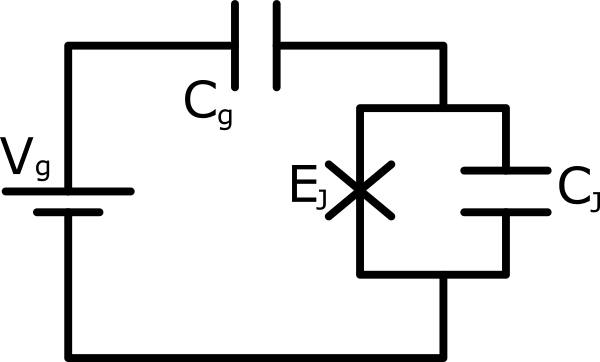
\includegraphics{Figures/CPB.png}
\decoRule
\caption[\CPB circuit]{The \CPB circuit with the \JJ represented as a bare \JJ with Josephson Energy $E_J$ and a capacitance $C_j$.}
\label{fig:cooperpairbox}
\end{figure}

The electrical energy of this circuit is the energy stored in the 2 capacitors, $C_g$ and $C_j$. If the total charge of the superconducting island is $-n|e|$, then the electrical energy ($\mathcal{H}_{el}$) is given by \cite{Schuster2007}
%---------------------------------------------------------
% Maybe you can show this in Appendix
%--------------------------------------------------------
\begin{equation}
\hat{\mathcal{H}_{el}}=4E_C(\hat{n}-n_g)^2
\end{equation}
where $\hat{n}\ket{n}=n\ket{n}$, $\ket{n}$ is the charge state with $n$ cooper pairs.\\
$E_C=e^2/2C_\Sigma=e^2/2(Cj+Cg)$ is the energy required to add one electron to the island and $n_g=C_gV_g/e$.\\
The energy levels are shown in Fig.\ref{fig:CPB EJ=0} for $E_J=0$. The \JJ would allow charge to tunnel through at $n_g=0.5,-0.5,1.5,-1.5\ldots$ in order to maintain the lowest energy.

\begin{figure}
\centering
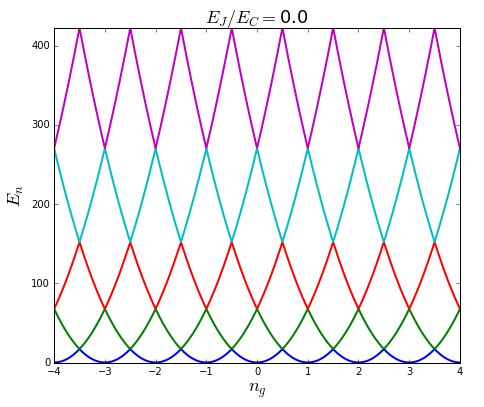
\includegraphics[width=300pt]{Figures/EjEc=0.png}
\decoRule
\caption[Energy Level for $E_J=0$]{Energy levels for $E_J=0$ or no tunneling. This figure was generated using \cite{Johansson2012}.}
\label{fig:CPB EJ=0}
\end{figure}

However, to calculate the complete Hamiltonian, we must also take into account the energy of the bare \JJ ($H_J$) which is given by.
\begin{equation}
\hat{\mathcal{H}_J}=-E_J\cos\hat{\delta}
\end{equation}
This is the tunnelling energy in the phase basis. To find the expression in the charge basis, we start with the commutation relation between charge and phase (See Appendix 1-A-2 from \cite{Cottet2002d}).
\begin{align}
\left[\hat{n},\hat{\delta}\right]&=-j
\label{eqn:commutation}
\end{align}
Using \ref{eqn:commutation} and the commutator identity \ref{eqn:comm identity}, we get
\begin{align}
\left[\hat{n},\hat{\delta}^m\right]&=\hat{\delta}^{m-1}\left[\hat{n},\hat{\delta}\right]+\hat{\delta}\left[\hat{n},\hat{\delta}^{m-1}\right]
\label{eqn:comm identity}\\
\end{align}
we can recursively use this relation to get
\begin{align}
\left[\hat{n},\hat{\delta}^m\right]&=-jm(\hat{\delta})^{m-1}\\
\hat{n}\hat{\delta}^m&=-jm\hat{\delta}^{m-1}+\hat{\delta}^m\hat{n}
\end{align}
The operator $\hat{n}e^{jp\hat{\delta}}$, where $p\in Z$, after expansion is
\begin{align}
\begin{split}
\hat{n}e^{jp\hat{\delta}}&=\hat{n}\sum_{m=0}^\infty \frac{( jp\hat{\delta})^m}{m!}=\sum_{m=0}^\infty \frac{(jp)^m\hat{n}\hat{\delta}^m}{m!}\\
&=\sum_{m=0}^\infty \frac{(jp)^m\hat{n}(\hat{\delta})^m}{m!}\\
&=\sum_{m=0}^\infty \frac{(jp)^m(-jm\hat{\delta}^{m-1}+\hat{\delta}^m\hat{n})}{m!}\\
&=\sum_{m=0}^\infty \frac{(jp)^m(-jm\hat{\delta}^{m-1})}{m!}+\sum_{m=0}^\infty \frac{(jp\hat{\delta})^m\hat{n}}{m!}\\
&=p\sum_{m=1}^\infty \frac{(jp\hat{\delta})^{m-1}}{(m-1)!}+\sum_{m=0}^\infty \frac{(jp\hat{\delta})^m\hat{n}}{m!}
\end{split}\\
\hat{n}e^{jp\hat{\delta}}&=pe^{jp\hat{\delta}}+e^{jp\hat{\delta}}\hat{n}
\end{align}
Using this operator on the charge state $\ket{n}$ gives
\begin{align}
\hat{n}\lbrace e^{jp\hat{\delta}}\ket{n}\rbrace&=pe^{jp\hat{\delta}}\ket{n}+e^{jp\hat{\delta}}\hat{n}\ket{n}\\
&=(n+p)\lbrace e^{jp\hat{\delta}}\ket{n}\rbrace\\
\implies e^{jp\hat{\delta}}\ket{n}&=\ket{n+p}
\end{align}
So, we can see that
\begin{align}
e^{ip\hat{\delta}}&=\sum_{m=-\infty}^\infty \ket{m+p}\bra{m}\\
\begin{split}
\cos\hat{\delta}=\frac{1}{2}\left(e^{i\hat{\delta}}+e^{-i\hat{\delta}}\right)&=\frac{1}{2}\left(\sum_{m=-\infty}^\infty \ket{m+1}\bra{m}+\sum_{m=-\infty}^\infty \ket{m-1}\bra{m}\right)\\
&=\frac{1}{2}\sum_{n=-\infty}^{+\infty}\ket{n}\bra{n+1}+\ket{n+1}\bra{n}
\end{split}
\end{align}
\begin{equation}
\hat{\mathcal{H}}_J=-\frac{E_J}{2}\left(\sum_{n=-\infty}^{+\infty}\ket{n}\bra{n+1}+\ket{n+1}\bra{n}\right)
\end{equation} 

So the complete Hamiltonian in the charge basis is the sum of these
\begin{equation}
\hat{\mathcal{H}}=\sum_{n=-\infty}^{+\infty}\left(4E_C(\hat{n}-n_g)^2\ket{n}\bra{n}-\frac{E_J}{2}\ket{n}\bra{n+1}+\ket{n+1}\bra{n}\right)
\label{eqn:charge basis ham}
\end{equation}

In the phase basis we can replace $\hat{n}$ with $-i\dfrac{\partial}{\partial\delta}$ to get
\begin{equation}
\hat{\mathcal{H}}=4E_C\left(-i\frac{\partial}{\partial\delta}-n_g\right)^2-E_J\cos\delta
\end{equation}

The energy eigenstates $\ket{k}$ are given by the schr\"{o}dinger equation
\begin{equation}
\hat{\mathcal{H}}(n_g)\ket{k}=E_k(n_g)\ket{k}
\end{equation}

These eigenenergies can be solved analytically in the phase basis in terms of Mathieu functions. The eigenenergies are given by
\begin{equation}
E_k(n_g)=E_Ca_{2[n_g+k(m,n_g)]}(-E_J/2E_C)
\end{equation}
where $a_\nu(q)$ denotes Mathieu’s characteristic value, and $k(m,n_g)$ is a function appropriately sorting the eigenvalues \cite{Koch2007a}.

\section{The 3D Superconducting Transmon}

A Transmon is basically a \CPB in which the \JJ is shunted with a large capacitance in order to decrease $E_C$ and so increase $E_J/E_C$.

The energy levels ($E_k$) plotted against gate charge ($n_g$) for different $E_J/E_C$ values are shown in Fig.\ref{fig:diff EJ/EC}.

\begin{figure}
\centering
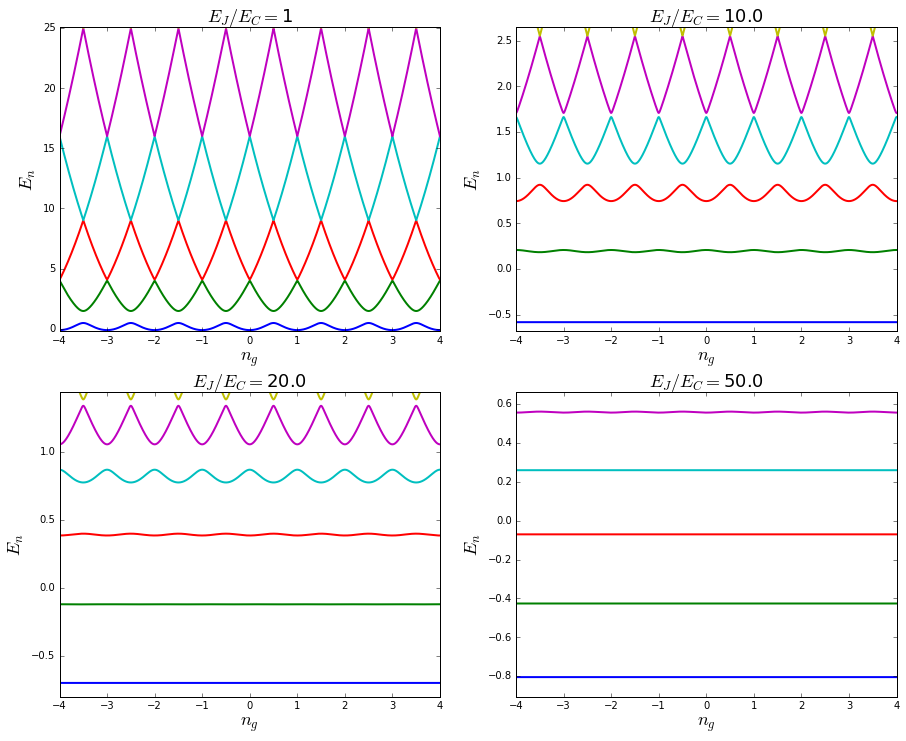
\includegraphics[width=\linewidth]{Figures/EjEcall.png}
\decoRule
\caption[Different $E_J/E_C$]{Energy levels for different $E_J/E_C$ values. Charge noise goes to zero as $E_J/E_C$ increases. Anharmonicity is also low but non-zero. This figure was generated using \cite{Johansson2012}.}
\label{fig:diff EJ/EC}
\end{figure}

As we can see the charge noise is very low for the case of high $E_J/E_C$. Also, anharmonicity, which is defined as $\alpha_h=E_{21}-E_{10}$, is reduced but not zero. In-fact, charge noise reduces exponentially while anharmonicity reduces only algebraically as $E_J/E_C$ is increased. This is the basis on which the transmon qubit is realised.

The Hamiltonian can also be solved using perturbation theory in the limit $E_J/E_C\gg 1$ by expanding the cosine in the tunnelling energy up to fourth order and treating the fourth order term as a perturbation. There is no dependence on $n_g$ because the system is charge insensitive at high $E_J/E_C$. The energy levels are \cite{Koch2007a}

\begin{equation}
E_k\approx-E_J+\sqrt{8E_CE_J}\left(k+\frac{1}{2}\right)-\frac{E_C}{12}(6k^2+6k+3)
\label{eqn:transmon levels}
\end{equation}

From \ref{eqn:transmon levels} we can see that the qubit transition frequency ($\omega_{10}$) is
\begin{equation}
\omega_{10}=\frac{E_1-E_0}{\hbar}=\frac{\sqrt{8E_JE_C}-E_C}{\hbar}
\end{equation}
and the anharmonicity
\begin{equation}
\alpha_h=(E_2-E_1)-(E_1-E_0)=-E_C
\end{equation}

\section{Coupling the Transmon to a Resonator}

For qubit readout and control, we will couple the qubit to a microwave cavity resonator (A rectangular waveguide resonator in this case). The lumped element circuit model of the qubit and cavity resonator is shown in Fig.\ref{fig:transmon with cavity}.

\begin{figure}
\centering
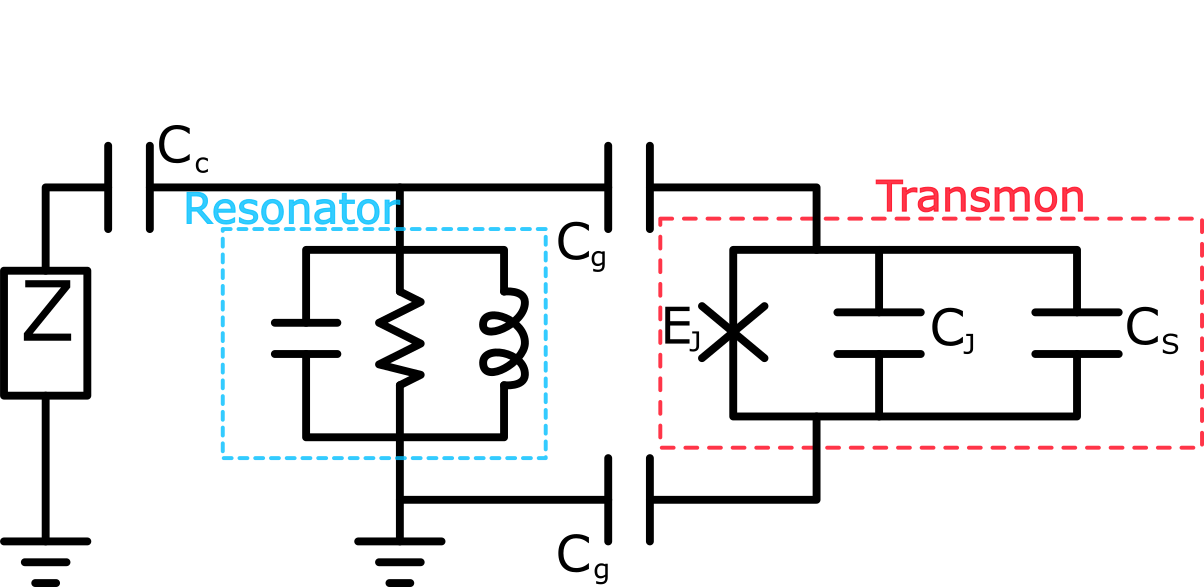
\includegraphics[width=\linewidth]{Figures/transmon_circuit.png}
\decoRule
\caption[Transmon Circuit]{Transmon coupled to the resonator coupled to the measurement device.}
\label{fig:transmon with cavity}
\end{figure}

We can approximate the transmon as a 2 level system with a ground state $\ket{g}$ and excited state $\ket{e}$ for large anharmonicity. In this approximation, the Hamiltonian of the system is discussed below  \cite{Richer2013,Schuster2007}.
\begin{itemize}
\item The Hamiltonian of the transmon can be expressed as the following if we choose the coordinate system appropriately and the zero energy as the mean energy of the transmon
\begin{equation}
\hat{\mathcal{H}}_{qubit}=-\frac{\hbar\omega_q}{2}\sigma_z
\label{eqn:qubit free hamiltonian}
\end{equation}
\item The Hamiltonian of the resonator is the same as the one for  an LC oscillator \ref{eqn:harmonic hamiltonian}
\begin{equation}
\hat{\mathcal{H}}_{cavity}=\hbar\omega_ra^\dag a
\end{equation}
The ground state energy of $\hbar\omega_r/2$ has not been shown as it does not have any significance in qubit dynamics.
\item The interaction hamiltonian is given by 
\begin{equation}
\hat{\mathcal{H}}_{int}=\hbar g(a^\dag\sigma_-+a\sigma_+)
\end{equation}
where $g$ is the coupling constant, proportional to the amplitude of the signal. The rotating wave approximation is made here, ignoring terms with $a^\dag\sigma_+$ and $a\sigma_-$.
\end{itemize}

This gives us the Jaynes-Cummings Hamiltonian
\begin{equation}
\hat{\mathcal{H}}=\hbar\omega_ra^\dag a-\frac{\hbar\omega_q}{2}\sigma_z+\hbar g(a^\dag\sigma_-+a\sigma_+)
\end{equation}

The eigenstates for the coupled system are
\begin{subequations}
\label{eqn:coupled eigenstates}
\begin{align}
\ket{n,+} &= \cos\frac{\theta_n}{2}\ket{e}\ket{n}+\sin\frac{\theta_n}{2}\ket{g}\ket{n+1}\\
\ket{n,-} &= -\sin\frac{\theta_n}{2}\ket{e}\ket{n}+\cos\frac{\theta_n}{2}\ket{g}\ket{n+1}
\end{align}
\end{subequations}
with eigenenergies
\begin{equation}
E_{n\pm}=\hbar\omega_r n\pm\frac{\sqrt{\hbar^2\Delta^2+4g^2(n+1)}}{2}
\end{equation}
where $\Delta=\omega_r-\omega_q$ and
\begin{equation}
\theta_n = \tan^{-1}\left(\frac{2g\sqrt{n+1}}{\hbar \Delta}\right)
\end{equation}

\section{The Bloch Sphere}

A general pure state for a two level system can represented as
\begin{equation}
\ket{\psi} = c_0\ket{0}+c_1\ket{1}
\end{equation}
where $\ket{0}$ and $\ket{1}$ form an orthonormal basis. $c_0=|c_0|e^{j\phi_1}$ and $c_1=|c_1|e^{j\phi_2}$ are complex numbers with a constraint that $|c_0|^2+|c_1|^2 = 1$ due to normalization. Since one can only measure the phase difference $\phi = \phi_2-\phi_1$, the state can be represented as
\begin{equation}
\ket{\psi} = \cos\frac{\theta}{2}\ket{0}+e^{j\phi}\sin\frac{\theta}{2}\ket{1}
\end{equation}
with no loss of generality where $\theta= 2\cos^{-1}|c_0|=2\sin^{-1}|c_1|$.

This state can be represented on a sphere with spherical coordinates on the surface with radius $r = 1$. The $\ket{0}$,$\ket{1}$ and an arbitrary state is shown in the Bloch Sphere in Fig.\ref{fig:bloch rep}.

\begin{figure}
\centering
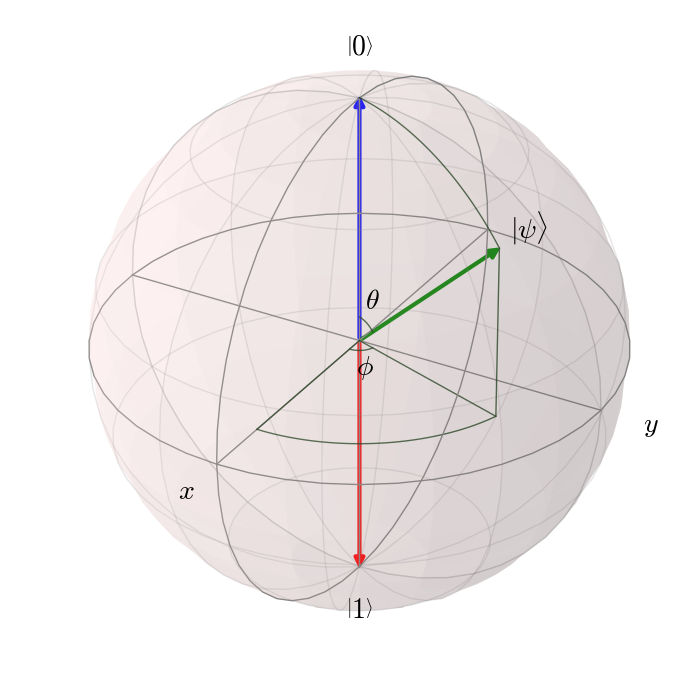
\includegraphics[width=\linewidth]{Figures/bloch_rep.png}
\decoRule
\caption[Bloch Sphere Representation]{Representation of states on a Bloch Sphere. The blue arrow represents the ground state $\ket{g}$, the red arrow represents the excited state $\ket{e}$, and the green arrow represents an arbitrary state $\ket{\psi} = \cos(\theta/2)\ket{g}+e^{j\phi}\sin(\theta/2)\ket{e}$.\\This figure was generated using \cite{Johansson2012}.}
\label{fig:bloch rep}
\end{figure}

\section{Dynamics of the Jaynes-Cummings system}

Let us consider the dynamics of the system in three different cases that are relevant to qubit manipulation and readout.
\begin{itemize}
\item \textbf{Zero Coupling} ($g=0$)\\
If there is no coupling (no photons in the cavity), then the qubit follows the free Hamiltonian given by \ref{eqn:qubit free hamiltonian}. The energy eigenstates of this system are $\ket{g}$ and $\ket{e}$ with energies $-\hbar\omega_q/2$ and $\hbar\omega_q/2$ respectively. In this basis, the Hamiltonian of the qubit can be expressed as
\begin{equation}
\hat{\mathcal{H}}_{qubit} = -\hbar\omega_q/2\ket{e}\bra{e} + \hbar\omega_q/2\ket{g}\bra{g}
\end{equation}
Applying the unitary operator $e^{i\hat{\mathcal{H}}t/\hbar}$ to an initial superposition state $\ket{\psi(0)}=c_0\ket{e}+c_1\ket{g}$ gives the state at a time $t$
\begin{align}
\begin{split}
\ket{\psi(t)} &= e^{i\hat{\mathcal{H}}t/\hbar}\ket{\psi(0)}\\
&=e^{-i\omega_qt/2}\left(c_0\ket{e}+e^{i\omega_q t}c_1{g}\right)
\end{split}
\end{align}

\begin{figure}
\centering
\begin{subfigure}[b]{0.45\textwidth}
\centering
\includegraphics[width=\textwidth]{Figures/rotatez.png}
%\decoRule
\caption{No Coupling}
\label{fig:rotatez}
\end{subfigure}
\hfill
\begin{subfigure}[b]{0.45\textwidth}
\centering
\includegraphics[width=\textwidth]{Figures/rotatex.png}
%\decoRule
\caption{On Resonance}
\label{fig:rotatex}
\end{subfigure}
\decoRule
\caption[Qubit Evolution on Bloch Sphere]{Evolution of an arbitrary state on the Bloch sphere. The light blue arrow represents the initial state and the dark blue arrow represents the final state. This figure was generated using \cite{Johansson2012}.}
\label{fig:rotatexz}
\end{figure}

We can see that if the qubit starts in an eigenstate, it remains in the same state (only a phase factor is added), but if it starts in a superposition, it's phase oscillates as a function of time with a frequency equal to the qubit frequency. On the bloch sphere this can be represented as a precession about the $z$-axis as shown in Fig.\ref{fig:rotatez}.

We can consider the dynamics of the coupled system in a similar way, once we change the basis to the new energy eigenstates in \ref{eqn:coupled eigenstates}.

\item \textbf{On Resonance} ($\Delta\ll g$)\\
If the drive signal or photons are at the same frequency as the qubit, then $\Delta=0$, which implies $\theta_n=\pi/2$. Then the eigenstates are
\begin{subequations}
\label{eqn:delta zero eigenstates}
\begin{align}
\ket{n,+} &= \frac{1}{\sqrt{2}}\ket{e}\ket{n}+\frac{1}{\sqrt{2}}\ket{g}\ket{n+1}\\
\ket{n,-} &= -\frac{1}{\sqrt{2}}\ket{e}\ket{n}+\frac{1}{\sqrt{2}}\ket{g}\ket{n+1}
\end{align}
\end{subequations}
With the new eigenstates, the qubit will oscillate about the $x$-axis as shown in Fig.\ref{fig:rotatex}. This means that if the initial state of the qubit is $\ket{g}$, it will oscillate to $\ket{e}$ in time $t=\pi g\sqrt{n+1}$. A pulsed signal which causes this transition\footnote{This signal refers to any signal which is resonant with the qubit and causes a rotation of $\pi$ radians about the $x$-axis on the Bloch Sphere.} is called a $\pi$-pulse The excitation number of the cavity will also oscillate from $\ket{n+1}$ to $\ket{n}$ with the same frequency.

It is worth noting that if the resonant frequency of the cavity is far from that of the qubit, and if the drive signal is of qubit frequency, then the qubit will still oscillate because it takes finite time for the photons to decay in the cavity.

\item \textbf{Low Power Dispersive limit} ($\Delta\gg g$)\\
In the low power dispersive limit\footnote{For the high power limit see \cite{Bishop2010}. The specific case of the transmon in the high power limit is discussed in \cite{Boissonneault2010}.}, the number of photons in the cavity is low ($\approx$ 1-100). We can rewrite the Hamiltonian by considering $g/\Delta$ as a perturbation since $\Delta\gg g$ \cite{Schuster2007} to get
\begin{equation}
\hat{\mathcal{H}}=\hbar\left(\omega_r+\frac{g^2}{\Delta}\sigma_z\right)a^\dag a+\frac{\hbar}{2}\left(\omega_q+\frac{g^2}{\Delta}\right)\sigma_z
\label{eqn:dispersive hamiltonian}
\end{equation}

\begin{figure}
\centering
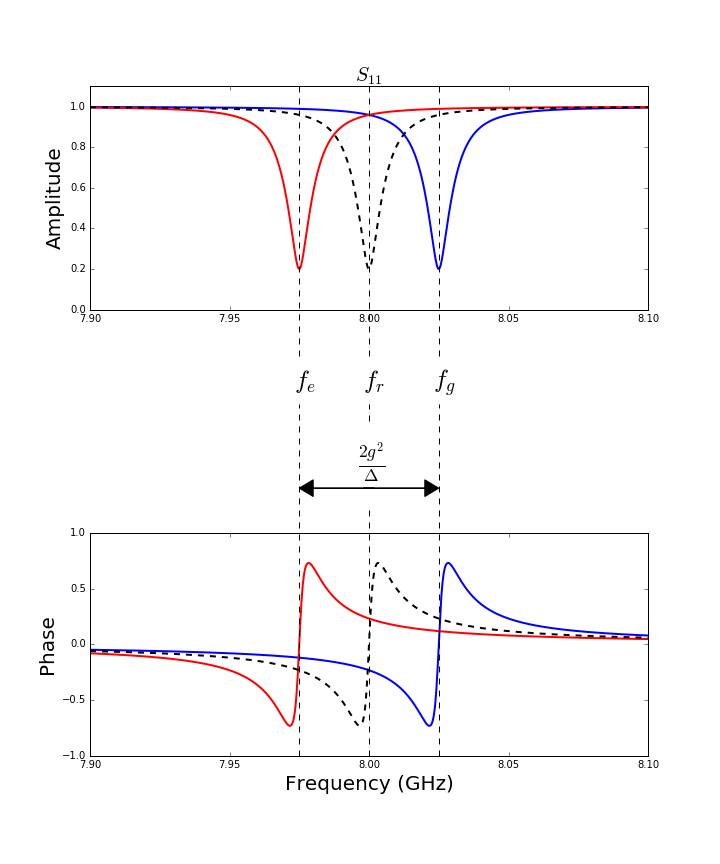
\includegraphics[width=\linewidth]{Figures/dispersive_shift.png}
\decoRule
\caption[Dispersive Shift]{Amplitude and Phase of $S_{11}$ for bare resonator (thick black dashed lines), resonator with qubit in ground state (thick blue line), and resonator with qubit in excited state (thick red line). The dispersive shift is $2g^2/\Delta$.}
\label{fig:dispersive shift}
\end{figure}

We can see from this Hamiltonian that dispersive coupling causes a shift of $\pm g^2/\Delta$ in the resonance frequency of the cavity depending on the qubit state. We can see the different $S_{11}$ parameter responses for the ground and excited states of the qubit in Fig.\ref{fig:dispersive shift}. This shift is crucial to measuring the state of the qubit.
We can also rearrange the equation as follows
\begin{equation}
\hat{\mathcal{H}}=\hbar\omega_r a^\dag a+\frac{\hbar}{2}\left(\omega_q+\frac{g^2}{\Delta}a^\dag a+\frac{g^2}{\Delta}\right)\sigma_z
\end{equation}
to see that the frequency of the qubit now has an added Lamb and ac-Stark shift of $g^2/\Delta$ and $g^2n/\Delta$ respectively \cite{Blais2004}.

The Hamiltonian in \ref{eqn:dispersive hamiltonian} can be written as
\begin{equation}
\hat{\mathcal{H}} = \hat{\mathcal{H}}_0 + \hat{\mathcal{H}}_{int}
\end{equation} 
where
\begin{equation}
\hat{\mathcal{H}}_0=\hbar\omega_r a^\dag a + \frac{\hbar\omega_q}{2} \sigma_z\
\end{equation}
is the uncoupled Hamiltonian of the qubit and cavity and
\begin{equation}
\hat{\mathcal{H}}_{int}=\frac{\hbar g^2\sigma_z}{\Delta}\left(a^\dag a+\frac{1}{2}\right)
\end{equation}
is the interaction Hamiltonian.\\

The unitary time evolution operator given by $\hat{U}(t)=e^{-j\hat{\mathcal{H}}t/\hbar}$ is
\begin{align}
\begin{split}
\hat{U}(t) = \text{exp}\left(-j\hat{\mathcal{H}}_0t/\hbar\right)\Bigg[&\text{ exp}\left(-j\frac{g^2t}{\Delta}\left(\hat{n}+\frac{1}{2}\right)\right)\ket{g}\bra{g}\\
+&\text{ exp}\left(j\frac{g^2t}{\Delta}\left(\hat{n}+\frac{1}{2}\right)\right)\ket{e}\bra{e}\Bigg]
\end{split}
\end{align}
If the initial state is such that the cavity is in a coherent state $\ket{\alpha}$ and the qubit is in a superposition state $(\ket{g}+\ket{e})/\sqrt{2}$, i.e
\begin{equation}
\ket{\psi(0)} = \frac{(\ket{g}+\ket{e})}{\sqrt{2}}\ket{\alpha}
\end{equation}
we can apply the unitary time evolution operator on this state and use the following relation
\begin{equation}
e^{i\varphi\hat{n}}\ket{\alpha} = \sum_{n=0}^\infty \frac{\alpha^ne^{i\varphi n}}{\sqrt{n!}}e^{-\frac{|\alpha|^2}{2}}\ket{n} = \ket{\alpha e^{i\varphi}}
\end{equation}
to get
\begin{align}
\begin{split}
\ket{\psi(t)} &= \hat{U}(t)\ket{\psi(0)}\\
&= \text{exp}\left(-j\hat{\mathcal{H}}_0t/\hbar\right)\frac{1}{\sqrt{2}}\Bigg[e^{-j\varphi/2}\ket{g}\ket{\alpha e^{-j\varphi}}+e^{j\varphi/2}\ket{e}\ket{\alpha e^{j\varphi}}\Bigg]
\end{split}
\end{align}
where $\varphi = g^2t/\Delta$. We can see that the cavity and qubit states are now entangled. The qubit ground state is entangled with the coherent state rotated by an angle $-\varphi$ and the excited state is entangled with the coherent state rotated by an angle $\varphi$.

At low powers, dispersive measurement is QND or Quantum Non-Demolition, which means that the qubit will remain in the eigenstate that was measured after a measurement. This means that repeated measurements will yield the same results.
\end{itemize}

\section{Decoherence}

A qubit which is initially in a superposition state $\ket{\psi} = \alpha\ket{g}+\beta\ket{e}$ will not stay in the superposition forever. It will lose its quantum information stochastically at a rate described below. The time for which the qubit retains its quantum information is called "coherence time", and is denoted by $T_2$. There are 2 processes which cause decoherence \cite{Geerlings2013}.
\begin{itemize}
\item \textbf{Relaxation}
The decay of the qubit to the ground state $\ket{g}$ due to spontaneous emission is referred to as relaxation. It does this at a rate $\Gamma_{\downarrow}$. If the qubit is in contact with a thermal bath at non zero temperature, there will also be excitation processes at a rate $\Gamma_{\uparrow}$. The combined effect gives the relaxation time $T_1 = \left(\Gamma_{\downarrow}+\Gamma_{\uparrow}\right)^{-1}$. Relaxation processes can be attributed to phenomena that cause energy fluctuations.
\item \textbf{Dephasing}
Dephasing is the process by which the qubit loses its phase information due to fluctuations is qubit frequency. These fluctuations cause the qubit to gain or lose phase and on average, lead to a diffused phase.
\end{itemize}

\section{Measurement Theory (Dispersive Limit)}

The setup for measurements is shown in Fig.\ref{fig:measurement setup}. All measurements described here assume that the cavity is dispersively coupled with the qubit. A signal of frequency $\omega_p$ is generated from port 1 of the VNA. This signal will be referred to as the probe signal. Another signal of frequency $\omega_d$ is combined with the probe signal and is sent into the cavity. This second signal is the drive signal. The VNA records the signal at port 2.

\begin{figure}
\centering
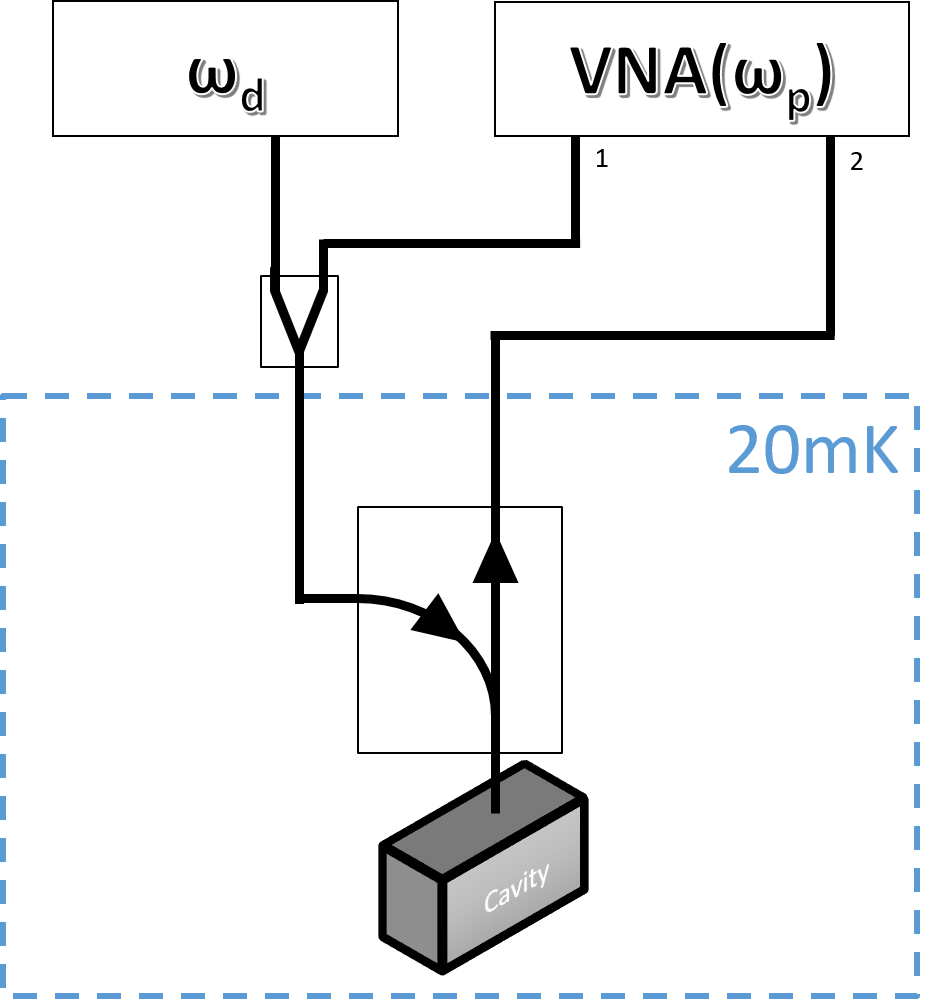
\includegraphics[width=400px]{Figures/measurement_circuit.png}
\decoRule
\caption[Measurement Setup]{Measurement Setup. The probe signal from the VNA and the drive signal from the signal generator is combined using a power combiner.}
\label{fig:measurement setup}
\end{figure}

\subsection{Single tone measurement}

In this measurement the drive signal is switched off and only the probe signal is sent to the cavity. We can plot the amplitude as a function of power and frequency of this signal. During this measurement, the qubit remains in the ground state except at high powers. This measurement was performed in \cite{Paik2011} with a 3D Transmon. The result of this measurement is similar to the ground state measurement in \cite{Reed2010}.

If the qubit is excited with a $\pi$-pulse at every point (i.e. for each frequency and power) and the amplitude is recorded for a certain period of time ($\approx$ 400 ns) and averaged, we can see the response of both the ground state and excited states. This experiment was performed in \cite{Reed2010} with a 2D Transmon.

\begin{itemize}
\item \textbf{Low Power Measurement}

The resonance occurs at the dispersively shifted frequency for low powers as expected.

\item \textbf{High Power Measurement}

At high powers, the resonance shifts toward the bare cavity frequency. This is described as a bright state of the cavity and is discussed in \cite{Bishop2010}. The specific case of the transmon is discussed in \cite{Boissonneault2010} where the transmon is treated as a Multi Level System.
\end{itemize}


\subsection{Two tone measurement}

Both the probe signal and drive signal are applied continuously in this measurement. The probe frequency is close to the cavity frequency and is used to populate the cavity with photons. The drive frequency is close to the qubit frequency and is used to manipulate the qubit. Application of the drive frequency exactly at the qubit frequency will cause the qubit to leave the ground state. If this drive tone is applied continuously, the qubit will have an equal probability of being in the ground and excited state, so there will be no dispersive shift.

Varying the frequencies and powers of the two signals can produce useful results.
\begin{itemize}
\item By probing the cavity with a fixed low power and a frequency equal to the cavity frequency, while varying the frequency of the drive signal at constant power, we can see a phase shift in the signal when the drive tone is at the qubit first transition frequency ($\omega_{01}$). For larger powers of the drive signal, the phase shift is larger. At sufficiently large powers, we can also see the qubit transition to the second excited level at $\omega_{12}$.
\item If the drive signal is swept at a constant power and the probe power is increased, we can see the qubit frequency changing as a result of ac-Stark shift as the number of photons in the cavity increase.
\item If the probe frequency is fixed close to the dispersively shifted resonance corresponding to one of the qubit states with a strong coupling rate and parameters such that $2\chi>\gamma,\kappa$, then spectroscopy with the drive frequency reveals the photon number state distribution in the cavity with different peaks corresponding to each photon number state. This is due to ac-Stark shift and is demonstrated using a \CPB in \cite{Schuster2007a}.
\end{itemize}

Details about Time Domain Measurements can be found in Appendix-\ref{AppendixB}
%\include{Chapters/Chapter4} 
%\include{Chapters/Chapter5}
%% Chapter 6

\chapter{Chapter Title Here} % Main chapter title

\label{Chapter6} % For referencing the chapter elsewhere, use \ref{Chapter1} 

%----------------------------------------------------------------------------------------

% Define some commands to keep the formatting separated from the content 
\newcommand{\keyword}[1]{\textbf{#1}}
\newcommand{\tabhead}[1]{\textbf{#1}}
\newcommand{\code}[1]{\texttt{#1}}
\newcommand{\file}[1]{\texttt{\bfseries#1}}
\newcommand{\option}[1]{\texttt{\itshape#1}}

%----------------------------------------------------------------------------------------

\section{Welcome and Thank You}
Welcome to this \LaTeX{} Thesis Template, a beautiful and easy to use template for writing a thesis using the \LaTeX{} typesetting system.

If you are writing a thesis (or will be in the future) and its subject is technical or mathematical (though it doesn't have to be), then creating it in \LaTeX{} is highly recommended as a way to make sure you can just get down to the essential writing without having to worry over formatting or wasting time arguing with your word processor.

\LaTeX{} is easily able to professionally typeset documents that run to hundreds or thousands of pages long. With simple mark-up commands, it automatically sets out the table of contents, margins, page headers and footers and keeps the formatting consistent and beautiful. One of its main strengths is the way it can easily typeset mathematics, even \emph{heavy} mathematics. Even if those equations are the most horribly twisted and most difficult mathematical problems that can only be solved on a super-computer, you can at least count on \LaTeX{} to make them look stunning.

%----------------------------------------------------------------------------------------

\section{Learning \LaTeX{}}

\LaTeX{} is not a \textsc{wysiwyg} (What You See is What You Get) program, unlike word processors such as Microsoft Word or Apple's Pages. Instead, a document written for \LaTeX{} is actually a simple, plain text file that contains \emph{no formatting}. You tell \LaTeX{} how you want the formatting in the finished document by writing in simple commands amongst the text, for example, if I want to use \emph{italic text for emphasis}, I write the \verb|\emph{text}| command and put the text I want in italics in between the curly braces. This means that \LaTeX{} is a \enquote{mark-up} language, very much like HTML.

\subsection{A (not so short) Introduction to \LaTeX{}}

If you are new to \LaTeX{}, there is a very good eBook -- freely available online as a PDF file -- called, \enquote{The Not So Short Introduction to \LaTeX{}}. The book's title is typically shortened to just \emph{lshort}. You can download the latest version (as it is occasionally updated) from here:
\url{http://www.ctan.org/tex-archive/info/lshort/english/lshort.pdf}

It is also available in several other languages. Find yours from the list on this page: \url{http://www.ctan.org/tex-archive/info/lshort/}

It is recommended to take a little time out to learn how to use \LaTeX{} by creating several, small `test' documents, or having a close look at several templates on:\\ 
\url{http://www.LaTeXTemplates.com}\\ 
Making the effort now means you're not stuck learning the system when what you \emph{really} need to be doing is writing your thesis.

\subsection{A Short Math Guide for \LaTeX{}}

If you are writing a technical or mathematical thesis, then you may want to read the document by the AMS (American Mathematical Society) called, \enquote{A Short Math Guide for \LaTeX{}}. It can be found online here:
\url{http://www.ams.org/tex/amslatex.html}
under the \enquote{Additional Documentation} section towards the bottom of the page.

\subsection{Common \LaTeX{} Math Symbols}
There are a multitude of mathematical symbols available for \LaTeX{} and it would take a great effort to learn the commands for them all. The most common ones you are likely to use are shown on this page:
\url{http://www.sunilpatel.co.uk/latex-type/latex-math-symbols/}

You can use this page as a reference or crib sheet, the symbols are rendered as large, high quality images so you can quickly find the \LaTeX{} command for the symbol you need.

\subsection{\LaTeX{} on a Mac}
 
The \LaTeX{} distribution is available for many systems including Windows, Linux and Mac OS X. The package for OS X is called MacTeX and it contains all the applications you need -- bundled together and pre-customized -- for a fully working \LaTeX{} environment and work flow.
 
MacTeX includes a custom dedicated \LaTeX{} editor called TeXShop for writing your `\file{.tex}' files and BibDesk: a program to manage your references and create your bibliography section just as easily as managing songs and creating playlists in iTunes.

%----------------------------------------------------------------------------------------

\section{Getting Started with this Template}

If you are familiar with \LaTeX{}, then you should explore the directory structure of the template and then proceed to place your own information into the \emph{THESIS INFORMATION} block of the \file{main.tex} file. You can then modify the rest of this file to your unique specifications based on your degree/university. Section \ref{FillingFile} on page \pageref{FillingFile} will help you do this. Make sure you also read section \ref{ThesisConventions} about thesis conventions to get the most out of this template.

If you are new to \LaTeX{} it is recommended that you carry on reading through the rest of the information in this document.

Before you begin using this template you should ensure that its style complies with the thesis style guidelines imposed by your institution. In most cases this template style and layout will be suitable. If it is not, it may only require a small change to bring the template in line with your institution's recommendations. These modifications will need to be done on the \file{MastersDoctoralThesis.cls} file.

\subsection{About this Template}

This \LaTeX{} Thesis Template is originally based and created around a \LaTeX{} style file created by Steve R.\ Gunn from the University of Southampton (UK), department of Electronics and Computer Science. You can find his original thesis style file at his site, here:
\url{http://www.ecs.soton.ac.uk/~srg/softwaretools/document/templates/}

Steve's \file{ecsthesis.cls} was then taken by Sunil Patel who modified it by creating a skeleton framework and folder structure to place the thesis files in. The resulting template can be found on Sunil's site here:
\url{http://www.sunilpatel.co.uk/thesis-template}

Sunil's template was made available through \url{http://www.LaTeXTemplates.com} where it was modified many times based on user requests and questions. Version 2.0 and onwards of this template represents a major modification to Sunil's template and is, in fact, hardly recognisable. The work to make version 2.0 possible was carried out by \href{mailto:vel@latextemplates.com}{Vel} and Johannes Böttcher.

%----------------------------------------------------------------------------------------

\section{What this Template Includes}

\subsection{Folders}

This template comes as a single zip file that expands out to several files and folders. The folder names are mostly self-explanatory:

\keyword{Appendices} -- this is the folder where you put the appendices. Each appendix should go into its own separate \file{.tex} file. An example and template are included in the directory.

\keyword{Chapters} -- this is the folder where you put the thesis chapters. A thesis usually has about six chapters, though there is no hard rule on this. Each chapter should go in its own separate \file{.tex} file and they can be split as:
\begin{itemize}
\item Chapter 1: Introduction to the thesis topic
\item Chapter 2: Background information and theory
\item Chapter 3: (Laboratory) experimental setup
\item Chapter 4: Details of experiment 1
\item Chapter 5: Details of experiment 2
\item Chapter 6: Discussion of the experimental results
\item Chapter 7: Conclusion and future directions
\end{itemize}
This chapter layout is specialised for the experimental sciences, your discipline may be different.

\keyword{Figures} -- this folder contains all figures for the thesis. These are the final images that will go into the thesis document.

\subsection{Files}

Included are also several files, most of them are plain text and you can see their contents in a text editor. After initial compilation, you will see that more auxiliary files are created by \LaTeX{} or BibTeX and which you don't need to delete or worry about:

\keyword{example.bib} -- this is an important file that contains all the bibliographic information and references that you will be citing in the thesis for use with BibTeX. You can write it manually, but there are reference manager programs available that will create and manage it for you. Bibliographies in \LaTeX{} are a large subject and you may need to read about BibTeX before starting with this. Many modern reference managers will allow you to export your references in BibTeX format which greatly eases the amount of work you have to do.

\keyword{MastersDoctoralThesis.cls} -- this is an important file. It is the class file that tells \LaTeX{} how to format the thesis. 

\keyword{main.pdf} -- this is your beautifully typeset thesis (in the PDF file format) created by \LaTeX{}. It is supplied in the PDF with the template and after you compile the template you should get an identical version.

\keyword{main.tex} -- this is an important file. This is the file that you tell \LaTeX{} to compile to produce your thesis as a PDF file. It contains the framework and constructs that tell \LaTeX{} how to layout the thesis. It is heavily commented so you can read exactly what each line of code does and why it is there. After you put your own information into the \emph{THESIS INFORMATION} block -- you have now started your thesis!

Files that are \emph{not} included, but are created by \LaTeX{} as auxiliary files include:

\keyword{main.aux} -- this is an auxiliary file generated by \LaTeX{}, if it is deleted \LaTeX{} simply regenerates it when you run the main \file{.tex} file.

\keyword{main.bbl} -- this is an auxiliary file generated by BibTeX, if it is deleted, BibTeX simply regenerates it when you run the \file{main.aux} file. Whereas the \file{.bib} file contains all the references you have, this \file{.bbl} file contains the references you have actually cited in the thesis and is used to build the bibliography section of the thesis.

\keyword{main.blg} -- this is an auxiliary file generated by BibTeX, if it is deleted BibTeX simply regenerates it when you run the main \file{.aux} file.

\keyword{main.lof} -- this is an auxiliary file generated by \LaTeX{}, if it is deleted \LaTeX{} simply regenerates it when you run the main \file{.tex} file. It tells \LaTeX{} how to build the \emph{List of Figures} section.

\keyword{main.log} -- this is an auxiliary file generated by \LaTeX{}, if it is deleted \LaTeX{} simply regenerates it when you run the main \file{.tex} file. It contains messages from \LaTeX{}, if you receive errors and warnings from \LaTeX{}, they will be in this \file{.log} file.

\keyword{main.lot} -- this is an auxiliary file generated by \LaTeX{}, if it is deleted \LaTeX{} simply regenerates it when you run the main \file{.tex} file. It tells \LaTeX{} how to build the \emph{List of Tables} section.

\keyword{main.out} -- this is an auxiliary file generated by \LaTeX{}, if it is deleted \LaTeX{} simply regenerates it when you run the main \file{.tex} file.

So from this long list, only the files with the \file{.bib}, \file{.cls} and \file{.tex} extensions are the most important ones. The other auxiliary files can be ignored or deleted as \LaTeX{} and BibTeX will regenerate them.

%----------------------------------------------------------------------------------------

\section{Filling in Your Information in the \file{main.tex} File}\label{FillingFile}

You will need to personalise the thesis template and make it your own by filling in your own information. This is done by editing the \file{main.tex} file in a text editor or your favourite LaTeX environment.

Open the file and scroll down to the third large block titled \emph{THESIS INFORMATION} where you can see the entries for \emph{University Name}, \emph{Department Name}, etc \ldots

Fill out the information about yourself, your group and institution. You can also insert web links, if you do, make sure you use the full URL, including the \code{http://} for this. If you don't want these to be linked, simply remove the \verb|\href{url}{name}| and only leave the name.

When you have done this, save the file and recompile \code{main.tex}. All the information you filled in should now be in the PDF, complete with web links. You can now begin your thesis proper!

%----------------------------------------------------------------------------------------

\section{The \code{main.tex} File Explained}

The \file{main.tex} file contains the structure of the thesis. There are plenty of written comments that explain what pages, sections and formatting the \LaTeX{} code is creating. Each major document element is divided into commented blocks with titles in all capitals to make it obvious what the following bit of code is doing. Initially there seems to be a lot of \LaTeX{} code, but this is all formatting, and it has all been taken care of so you don't have to do it.

Begin by checking that your information on the title page is correct. For the thesis declaration, your institution may insist on something different than the text given. If this is the case, just replace what you see with what is required in the \emph{DECLARATION PAGE} block.

Then comes a page which contains a funny quote. You can put your own, or quote your favourite scientist, author, person, and so on. Make sure to put the name of the person who you took the quote from.

Following this is the abstract page which summarises your work in a condensed way and can almost be used as a standalone document to describe what you have done. The text you write will cause the heading to move up so don't worry about running out of space.

Next come the acknowledgements. On this page, write about all the people who you wish to thank (not forgetting parents, partners and your advisor/supervisor).

The contents pages, list of figures and tables are all taken care of for you and do not need to be manually created or edited. The next set of pages are more likely to be optional and can be deleted since they are for a more technical thesis: insert a list of abbreviations you have used in the thesis, then a list of the physical constants and numbers you refer to and finally, a list of mathematical symbols used in any formulae. Making the effort to fill these tables means the reader has a one-stop place to refer to instead of searching the internet and references to try and find out what you meant by certain abbreviations or symbols.

The list of symbols is split into the Roman and Greek alphabets. Whereas the abbreviations and symbols ought to be listed in alphabetical order (and this is \emph{not} done automatically for you) the list of physical constants should be grouped into similar themes.

The next page contains a one line dedication. Who will you dedicate your thesis to?

Finally, there is the block where the chapters are included. Uncomment the lines (delete the \code{\%} character) as you write the chapters. Each chapter should be written in its own file and put into the \emph{Chapters} folder and named \file{Chapter1}, \file{Chapter2}, etc\ldots Similarly for the appendices, uncomment the lines as you need them. Each appendix should go into its own file and placed in the \emph{Appendices} folder.

After the preamble, chapters and appendices finally comes the bibliography. The bibliography style (called \option{authoryear}) is used for the bibliography and is a fully featured style that will even include links to where the referenced paper can be found online. Do not underestimate how grateful your reader will be to find that a reference to a paper is just a click away. Of course, this relies on you putting the URL information into the BibTeX file in the first place.

%----------------------------------------------------------------------------------------

\section{Thesis Features and Conventions}\label{ThesisConventions}

To get the best out of this template, there are a few conventions that you may want to follow.

One of the most important (and most difficult) things to keep track of in such a long document as a thesis is consistency. Using certain conventions and ways of doing things (such as using a Todo list) makes the job easier. Of course, all of these are optional and you can adopt your own method.

\subsection{Printing Format}

This thesis template is designed for double sided printing (i.e. content on the front and back of pages) as most theses are printed and bound this way. Switching to one sided printing is as simple as uncommenting the \option{oneside} option of the \code{documentclass} command at the top of the \file{main.tex} file. You may then wish to adjust the margins to suit specifications from your institution.

The headers for the pages contain the page number on the outer side (so it is easy to flick through to the page you want) and the chapter name on the inner side.

The text is set to 11 point by default with single line spacing, again, you can tune the text size and spacing should you want or need to using the options at the very start of \file{main.tex}. The spacing can be changed similarly by replacing the \option{singlespacing} with \option{onehalfspacing} or \option{doublespacing}.

\subsection{Using US Letter Paper}

The paper size used in the template is A4, which is the standard size in Europe. If you are using this thesis template elsewhere and particularly in the United States, then you may have to change the A4 paper size to the US Letter size. This can be done in the margins settings section in \file{main.tex}.

Due to the differences in the paper size, the resulting margins may be different to what you like or require (as it is common for institutions to dictate certain margin sizes). If this is the case, then the margin sizes can be tweaked by modifying the values in the same block as where you set the paper size. Now your document should be set up for US Letter paper size with suitable margins.

\subsection{References}

The \code{biblatex} package is used to format the bibliography and inserts references such as this one \parencite{Reference1}. The options used in the \file{main.tex} file mean that the in-text citations of references are formatted with the author(s) listed with the date of the publication. Multiple references are separated by semicolons (e.g. \parencite{Reference2, Reference1}) and references with more than three authors only show the first author with \emph{et al.} indicating there are more authors (e.g. \parencite{Reference3}). This is done automatically for you. To see how you use references, have a look at the \file{Chapter1.tex} source file. Many reference managers allow you to simply drag the reference into the document as you type.

Scientific references should come \emph{before} the punctuation mark if there is one (such as a comma or period). The same goes for footnotes\footnote{Such as this footnote, here down at the bottom of the page.}. You can change this but the most important thing is to keep the convention consistent throughout the thesis. Footnotes themselves should be full, descriptive sentences (beginning with a capital letter and ending with a full stop). The APA6 states: \enquote{Footnote numbers should be superscripted, [...], following any punctuation mark except a dash.} The Chicago manual of style states: \enquote{A note number should be placed at the end of a sentence or clause. The number follows any punctuation mark except the dash, which it precedes. It follows a closing parenthesis.}

The bibliography is typeset with references listed in alphabetical order by the first author's last name. This is similar to the APA referencing style. To see how \LaTeX{} typesets the bibliography, have a look at the very end of this document (or just click on the reference number links in in-text citations).

\subsubsection{A Note on bibtex}

The bibtex backend used in the template by default does not correctly handle unicode character encoding (i.e. "international" characters). You may see a warning about this in the compilation log and, if your references contain unicode characters, they may not show up correctly or at all. The solution to this is to use the biber backend instead of the outdated bibtex backend. This is done by finding this in \file{main.tex}: \option{backend=bibtex} and changing it to \option{backend=biber}. You will then need to delete all auxiliary BibTeX files and navigate to the template directory in your terminal (command prompt). Once there, simply type \code{biber main} and biber will compile your bibliography. You can then compile \file{main.tex} as normal and your bibliography will be updated. An alternative is to set up your LaTeX editor to compile with biber instead of bibtex, see \href{http://tex.stackexchange.com/questions/154751/biblatex-with-biber-configuring-my-editor-to-avoid-undefined-citations/}{here} for how to do this for various editors.

\subsection{Tables}

Tables are an important way of displaying your results, below is an example table which was generated with this code:

{\small
\begin{verbatim}
\begin{table}
\caption{The effects of treatments X and Y on the four groups studied.}
\label{tab:treatments}
\centering
\begin{tabular}{l l l}
\toprule
\tabhead{Groups} & \tabhead{Treatment X} & \tabhead{Treatment Y} \\
\midrule
1 & 0.2 & 0.8\\
2 & 0.17 & 0.7\\
3 & 0.24 & 0.75\\
4 & 0.68 & 0.3\\
\bottomrule\\
\end{tabular}
\end{table}
\end{verbatim}
}

\begin{table}
\caption{The effects of treatments X and Y on the four groups studied.}
\label{tab:treatments}
\centering
\begin{tabular}{l l l}
\toprule
\tabhead{Groups} & \tabhead{Treatment X} & \tabhead{Treatment Y} \\
\midrule
1 & 0.2 & 0.8\\
2 & 0.17 & 0.7\\
3 & 0.24 & 0.75\\
4 & 0.68 & 0.3\\
\bottomrule\\
\end{tabular}
\end{table}

You can reference tables with \verb|\ref{<label>}| where the label is defined within the table environment. See \file{Chapter1.tex} for an example of the label and citation (e.g. Table~\ref{tab:treatments}).

\subsection{Figures}

There will hopefully be many figures in your thesis (that should be placed in the \emph{Figures} folder). The way to insert figures into your thesis is to use a code template like this:
\begin{verbatim}
\begin{figure}
\centering

\includegraphics{Figures/Electron}
\decoRule
\caption[An Electron]{An electron (artist's impression).}
\label{fig:Electron}
\end{figure}
\end{verbatim}
Also look in the source file. Putting this code into the source file produces the picture of the electron that you can see in the figure below.

\begin{figure}[th]
\centering

\includegraphics{Figures/Electron}
\decoRule
\caption[An Electron]{An electron (artist's impression).}
\label{fig:Electron}
\end{figure}

Sometimes figures don't always appear where you write them in the source. The placement depends on how much space there is on the page for the figure. Sometimes there is not enough room to fit a figure directly where it should go (in relation to the text) and so \LaTeX{} puts it at the top of the next page. Positioning figures is the job of \LaTeX{} and so you should only worry about making them look good!

Figures usually should have captions just in case you need to refer to them (such as in Figure~\ref{fig:Electron}). The \verb|\caption| command contains two parts, the first part, inside the square brackets is the title that will appear in the \emph{List of Figures}, and so should be short. The second part in the curly brackets should contain the longer and more descriptive caption text.

The \verb|\decoRule| command is optional and simply puts an aesthetic horizontal line below the image. If you do this for one image, do it for all of them.

\LaTeX{} is capable of using images in pdf, jpg and png format.

\subsection{Typesetting mathematics}

If your thesis is going to contain heavy mathematical content, be sure that \LaTeX{} will make it look beautiful, even though it won't be able to solve the equations for you.

The \enquote{Not So Short Introduction to \LaTeX} (available on \href{http://www.ctan.org/tex-archive/info/lshort/english/lshort.pdf}{CTAN}) should tell you everything you need to know for most cases of typesetting mathematics. If you need more information, a much more thorough mathematical guide is available from the AMS called, \enquote{A Short Math Guide to \LaTeX} and can be downloaded from:
\url{ftp://ftp.ams.org/pub/tex/doc/amsmath/short-math-guide.pdf}

There are many different \LaTeX{} symbols to remember, luckily you can find the most common symbols in \href{http://ctan.org/pkg/comprehensive}{The Comprehensive \LaTeX~Symbol List}.

You can write an equation, which is automatically given an equation number by \LaTeX{} like this:
\begin{verbatim}
\begin{equation}
E = mc^{2}
\label{eqn:Einstein}
\end{equation}
\end{verbatim}

This will produce Einstein's famous energy-matter equivalence equation:
\begin{equation}
E = mc^{2}
\label{eqn:Einstein}
\end{equation}

All equations you write (which are not in the middle of paragraph text) are automatically given equation numbers by \LaTeX{}. If you don't want a particular equation numbered, use the unnumbered form:
\begin{verbatim}
\[ a^{2}=4 \]
\end{verbatim}

%----------------------------------------------------------------------------------------

\section{Sectioning and Subsectioning}

You should break your thesis up into nice, bite-sized sections and subsections. \LaTeX{} automatically builds a table of Contents by looking at all the \verb|\chapter{}|, \verb|\section{}|  and \verb|\subsection{}| commands you write in the source.

The Table of Contents should only list the sections to three (3) levels. A \verb|chapter{}| is level zero (0). A \verb|\section{}| is level one (1) and so a \verb|\subsection{}| is level two (2). In your thesis it is likely that you will even use a \verb|subsubsection{}|, which is level three (3). The depth to which the Table of Contents is formatted is set within \file{MastersDoctoralThesis.cls}. If you need this changed, you can do it in \file{main.tex}.

%----------------------------------------------------------------------------------------

\section{In Closing}

You have reached the end of this mini-guide. You can now rename or overwrite this pdf file and begin writing your own \file{Chapter1.tex} and the rest of your thesis. The easy work of setting up the structure and framework has been taken care of for you. It's now your job to fill it out!

Good luck and have lots of fun!

\begin{flushright}
Guide written by ---\\
Sunil Patel: \href{http://www.sunilpatel.co.uk}{www.sunilpatel.co.uk}\\
Vel: \href{http://www.LaTeXTemplates.com}{LaTeXTemplates.com}
\end{flushright}
 


%----------------------------------------------------------------------------------------
%	THESIS CONTENT - APPENDICES
%----------------------------------------------------------------------------------------

\appendix % Cue to tell LaTeX that the following "chapters" are Appendices

% Include the appendices of the thesis as separate files from the Appendices folder
% Uncomment the lines as you write the Appendices

% Appendix A

\chapter{Calculation of Required Junction Resistance} % Main appendix title

\label{AppendixA} % For referencing this appendix elsewhere, use \ref{AppendixA}

If the capacitive pads of the transmon have a $70$fF shunt capacitance ($C_s$)\footnote{The shunt capacitance $C_s$ is also the dominating capacitance for a junction with small area ($C_s\gg C_j$)} as in \cite{Paik2011}, then the charging energy is
\begin{equation}
\frac{E_C}{h} = \frac{e^2}{2C_\Sigma}= \frac{e^2}{2*\SI{70}{\femto \farad}} = \SI{0.277056}{\giga\hertz}
\end{equation}

To construct a $\SI{7}{\giga\hertz}$ qubit, $E_2-E_1 = \sqrt{8E_JE_C}-E_C = h\SI{7}{\giga\hertz}$. Then the Junctiion energy is
\begin{equation}
\frac{E_J}{h} = \frac{(h\times\SI{7}{\giga\hertz}+E_C)^2}{8E_C} = \SI{23.89}{\giga\hertz}
\end{equation}

The critical current for a given $E_J$ can be calculated using \ref{eqn:junction energy}.
\begin{equation}
I_0 = \frac{2eE_J}{\hbar} = \SI{46.2442}{\nano\ampere}
\end{equation}

The Juntion Resistance ($R_N$) can be calculated using the Ambegaokar-Baratoff formula
\begin{equation}
I_0 = \frac{\pi\Delta_s}{2eR_N}\tanh\frac{\Delta_s}{2k_BT}
\end{equation}
where $k_B$ is the Boltzmann Constant and $\Delta_s$ is the superconducting gap, which in this case is that of aluminium. This can be calculated using BCS theory as
\begin{equation}
\Delta_s = 1.764\times k_BT_C
\end{equation}
where $T_C = \SI{1.1}{K}$ si the critical temperature of aluminium.

In the zero temperature limit, the junction resistance $R_N$ is given by
\begin{equation}
R_N = \frac{\pi\Delta_s}{2eI_0} = \SI{5.68188}{\kilo\ohm}
\end{equation}

The junction inductance can also be calculated as
\begin{equation}
L_J = \frac{\Phi_0}{I_0} = \frac{\hbar}{2eI_0} = \SI{7.09833}{\nano\henry}
\end{equation}

% Appendix Template

\chapter{Time Domain Measurements} % Main appendix title

\label{AppendixB} % Change X to a consecutive letter; for referencing this appendix elsewhere, use \ref{AppendixX}

The time domain measurements involve recording the reflected probe signal of the probe signal which is used to populate the cavity with photons.\\The drive signal or control signal of frequency equal to the qubit frequency will be sent in pulses in order to manipulate the qubit.\\The Measurement tone is sent and it's quadrature components are recorded continuously as a function of time. The method of measurement is well described and demonstrated in \cite{Bianchetti2009}.

\begin{itemize}
\item \textbf{Cavity Decay Time}

This measurement involves sending a microwave pulse to populate the cavity with photons, and then measure the cavity response as a function of time. This is a ring down measurement since it involves the cavity losing photons and coming down to the zero-photon\footnote{This refers to the experiment done at milli-Kelvin temperatures. Ring down measurement can also be done at higher temperatures, where the photon number comes down to thermal equilibrium} state. The cavity response shows an exponential decay, and the time taken for the response to reduce by a factor of $1/e$ is the cavity decay time $1/\kappa$.

\item \textbf{Rabi Measurement}

This measurement is used to calibrate the length of a pi-pulse. The qubit is initialized in ground state\footnote{This is done by waiting long enough so the qubit relaxes to ground state.}. A pulse of length $\Delta\tau$ and frequency $\omega_q$ is sent to the cavity and then the cavity response is measured (ring-down for example)\footnote{A continuous measurement scheme is described in \cite{Bianchetti2009}}. This measurement is repeated multiple times and the average is taken. The area between the measured curve (IQ values) for an arbitrary state and the ground state is proportional to the excitation probability of the qubit.

Plotting the excitation probabilities as a function of $\Delta\tau$ shows an oscillating behaviour. The pulse time for a pi pulse, which is $\Delta\tau$ for which the first peak in excitation probability is observed, is calibrated using this measurement.

\item \textbf{Relaxation Time}

The experiment for finding the relaxation time $T_1$ for the qubit involves first exciting the qubit using a pi pulse, and measuring the cavity response after waiting for a time $\Delta t$. Plotting the excited state probability vs $\Delta t$ shows an exponential decay. The time $\Delta t$ at which the excitation probability drops to $1/e$ of the initial probability is the relaxation time $T_1$.
\end{itemize}
%\include{Appendices/AppendixC}

%----------------------------------------------------------------------------------------
%	BIBLIOGRAPHY
%----------------------------------------------------------------------------------------

\printbibliography[heading=bibintoc]

%----------------------------------------------------------------------------------------

\end{document}  
